%%%%%%%%%%%%%%%%%%%%%%%%%%%%%%%%%%%%%%%%%%%%%%%%%%%%%%
%
% This file defines the style for your report.
%
% Just run "sh compiletex.sh" to compile
% 
%%%%%%%%%%%%%%%%%%%%%%%%%%%%%%%%%%%%%%%%%%%%%%%%%%%%%%

\documentclass[10pt,  english, makeidx, a4paper, titlepage, oneside]{book}
\usepackage{babel}
\usepackage{fancyhdr}
\usepackage{makeidx}
\usepackage{titlesec}
\usepackage{listings}
\usepackage{booktabs}
\usepackage{hyperref}
\usepackage{caption}
\usepackage{subcaption}


\newenvironment{listato}{\footnotesize}{\normalsize }

\textwidth 15.5cm
\textheight 23cm
\topmargin -1cm
\oddsidemargin -0.5cm
\linespread{1.1}

\pagestyle{fancy}
\lhead{}
\chead{Cybersecurity for Embedded Systems}
\lfoot{}
\cfoot{}
\rfoot{}
\rhead{\thepage}

\usepackage{graphicx}
\usepackage{amsmath}
\usepackage{amsfonts}
\usepackage{amsthm}
\usepackage{amssymb}
\usepackage{graphicx}
\usepackage{caption}
\usepackage{float}
\usepackage{amsmath}
\usepackage{amssymb}
\usepackage{amsfonts}
\usepackage{amsthm}
\usepackage{empheq}
\usepackage{verbatim}
\usepackage{fancyvrb}
\usepackage[dvipsnames]{xcolor}


\definecolor{codegreen}{rgb}{0,0.6,0}
\definecolor{codegray}{rgb}{0.5,0.5,0.5}
\definecolor{codepurple}{rgb}{0.58,0,0.82}
\definecolor{backcolour}{rgb}{0.95,0.95,0.92}

\lstdefinestyle{mystyle}{
    backgroundcolor=\color{backcolour},   
    commentstyle=\color{codegreen},
    keywordstyle=\color{magenta},
    numberstyle=\tiny\color{codegray},
    stringstyle=\color{codepurple},
    basicstyle=\ttfamily\footnotesize,
    breakatwhitespace=false,         
    breaklines=true,                 
    captionpos=b,                    
    keepspaces=true,                 
    numbers=left,                    
    numbersep=5pt,                  
    showspaces=false,                
    showstringspaces=false,
    showtabs=false,                  
    tabsize=2
}

\lstdefinelanguage{Kotlin}{
  comment=[l]{//},
  commentstyle={\color{gray}\ttfamily},
  emph={filter, first, firstOrNull, forEach, lazy, map, mapNotNull, println},
  emphstyle={\color{OrangeRed}},
  identifierstyle=\color{black},
  keywords={!in, !is, abstract, actual, annotation, as, as?, break, by, catch, class, companion, const, constructor, continue, crossinline, data, delegate, do, dynamic, else, enum, expect, external, false, field, file, final, finally, for, fun, get, if, import, in, infix, init, inline, inner, interface, internal, is, lateinit, noinline, null, object, open, operator, out, override, package, param, private, property, protected, public, receiveris, reified, return, return@, sealed, set, setparam, super, suspend, tailrec, this, throw, true, try, typealias, typeof, val, var, vararg, when, where, while},
  keywordstyle={\color{NavyBlue}\bfseries},
  morecomment=[s]{/*}{*/},
  morestring=[b]",
  morestring=[s]{"""*}{*"""},
  ndkeywords={@Deprecated, @JvmField, @JvmName, @JvmOverloads, @JvmStatic, @JvmSynthetic, Array, Byte, Double, Float, Int, Integer, Iterable, Long, Runnable, Short, String, Any, Unit, Nothing},
  ndkeywordstyle={\color{BurntOrange}\bfseries},
  sensitive=true,
  stringstyle={\color{ForestGreen}\ttfamily},
}

\lstset{style=mystyle}

\titleformat{\chapter}[display]
{\normalfont\Large\filcenter\sffamily}
{\titlerule[0.5pt]%
\vspace{1pt}
\titlerule
\vspace{1pc}
\LARGE\MakeUppercase{\chaptertitlename} \thechapter
}
{1pc}
{\titlerule
\vspace{1pc}
\Huge}

\makeindex

\begin{document}

\frontmatter
\begin{titlepage}
\vspace{0cm}
\centerline{

\includegraphics[width=6cm]{./logopolitonuovo}} 
\vspace{0.5cm}
\centerline{\LARGE Politecnico di Torino}
\vspace{2.5cm}
\centerline{\huge Cybersecurity for Embedded Systems}
\vspace{0.25cm}
\centerline{\huge 01UDNOV}
\vspace{1cm}
\centerline{\Large Master's Degree in Computer Engineering}
\vspace{2.5cm}
\centerline{\Huge Live Audio Watermarking}
\bigskip
\centerline{\huge Project Report}
\vspace{2cm}
\vfill
\begin{minipage}{6.5cm} % modify this width in order to keep everything on the same line
\Large{Candidates:\\
Lorenzo Marino (317703)\\
Agostino Saviano (307946)\\
Niccolò Cacioli (305325)}
\end{minipage}
\hfill
\begin{minipage}{4.4cm}
\Large{Referee: \\
Prof. Paolo Prinetto}
\end{minipage}
\end{titlepage}

\tableofcontents
\listoffigures % REMOVE THIS IF THERE ARE NO PICTURES
\listoftables % REMOVE THIS IF THERE ARE NO TABLES

\mainmatter
    
% HERE IS WHERE YOU INCLUDE YOUR CHAPTERS

\chapter*{Abstract}
With an increasing level of technology and an even higher progress of AI, attacking the credibility of high level positions has become more frequent and therefore assuring the authenticity of recorded conversations has also become way more important.


Here can be read how Watermarking can be properly used to guarantee the integrity of data sent over voice communication as a possible solution for this kind of problem.
Watermarking allows to embed data into a signal and by doing this the author can eventually sign the data and certify the ownership of a communication.


Another useful tool descripted in this paper is the usage of high frequencies as a possible improvement to be able to operate and assure the properties of the signal through an inaudible range of the human hearing, thus being able to not interfere with a normal conversation and also to discreetly defend the talker itself.


Both these concepts have been studied and applied in order to propose a demo of an application that can be used to apply a watermark to a nearby recording microphone, implementing an easier and naive version, although still relevant and practical for this project.


Live watermarking can be a solution to prevent malicious attackers from counterfeiting and misusing simple voice commands or personal sensitive chats and this paper provides an all around guide to start studying these topics.




%This is the space reserved for the abstract of your report. The abstract is a summary of the report, so it is a good idea to write after all other chapters. The abstract for a thesis at PoliTO must be shorter than 3500 chars, try to be compliant with this rule (no problem for an abstract that is a lot shorter than 3500 chars, since this is not a thesis).
%Use short sentences, do not use over-complicated words. Try to be as clear as possible, do not make logical leaps in the text. Read your abstract several times and check if there is a logical connection from the beginning to the end. The abstract is supposed to draw the attention of the reader, your goal is to write an abstract that makes the reader wanting to read the entire report. Do not go too far into details; if you want to provide data, do it, but express it in a simple way (e.g., a single percentage in a sentence): do not bore the reader with data that he or she cannot understand yet. Organize the abstract into paragraphs: the paragraphs are always 3 to 5 lines long. In \LaTeX source file, go new line twice to start a new paragraph in the PDF. Do not use $\\$ to go new line, just press Enter. In the PDF, there will be no gap line, but the text will go new line and a Tab will be inserted. This is the correct way to indent a paragraph, please do not change it. Do not put words in \textbf{bold} here: for emphasis, use \emph{italic}. Do not use citations here: they are not allowed in the abstract. Footnotes and links are not allowed as well. DO NOT EVER USE ENGLISH SHORT FORMS (i.e., isn't, aren't, don't, etc.).
%Take a look at the following links about how to write an Abstract:
%\begin{itemize}
%\item \url{https://writing.wisc.edu/handbook/assignments/writing-an-abstract-for-your-research-paper/}
%\item \url{https://www.anu.edu.au/students/academic-skills/research-writing/journal-article-writing/writing-an-abstract}
%\end{itemize}
%Search on Google if you need more info.
\graphicspath{ {LiveAudioWatermarking/Images/} }
\chapter{Introduction}
The goal of this chapter is to introduce the main technologies that are used to build a modern microphone: MEMS and ECM. 


In the next chapter the watermarking procedure will be described in detail and how such technique helped to implement the use case of the project. \newline
Chapter 3 describes the state of the art of modern day attacks and then in the last chapters the implementation and the results of the project will be discussed.
\section{State of the Art: MEMS and ECM}
\subsection{MEMS Microphone}
MEMS (Micro-Electro-Mechanical System) Microphones use a MEMS component placed on a printed circuit board (PCB) and protected with a mechanical cover. A small hole is fabricated in the case to allow sound into the microphone and is either designated as top-ported if the hole is in the top cover or bottom-ported if the hole is in the PCB. The MEMS component is often designed with a mechanical diaphragm and mounting structure created on a semiconductor die.
\subsection{How it works}
The MEMS diaphragm forms a capacitor and sound pressure waves cause movement of the diaphragm. MEMS microphones typically contain a second semiconductor die which functions as an audio preamplifier, converting the changing capacitance of the MEMS to an electrical signal. The output of the audio preamplifier is provided to the user if an analog output signal is desired. If a digital output signal is desired, then an analog-to-digital converter (ADC) is included on the same die as the audio preamplifier. A common format used for the digital encoding in MEMS microphones is pulse density modulation (PDM), which allows for communication with only a clock and a single data line. Decoding of the digital signal at the receiver is simplified due to the single bit encoding of the data. Digital I²S outputs are a third option that include an internal decimation filter, which allows for processing to be completed in the microphone itself. This means the microphone can connect directly to a digital signal processor (DSP) or microcontroller, eliminating the need for an ADC or codec in many applications.
\begin{figure}[H]
    \centering
    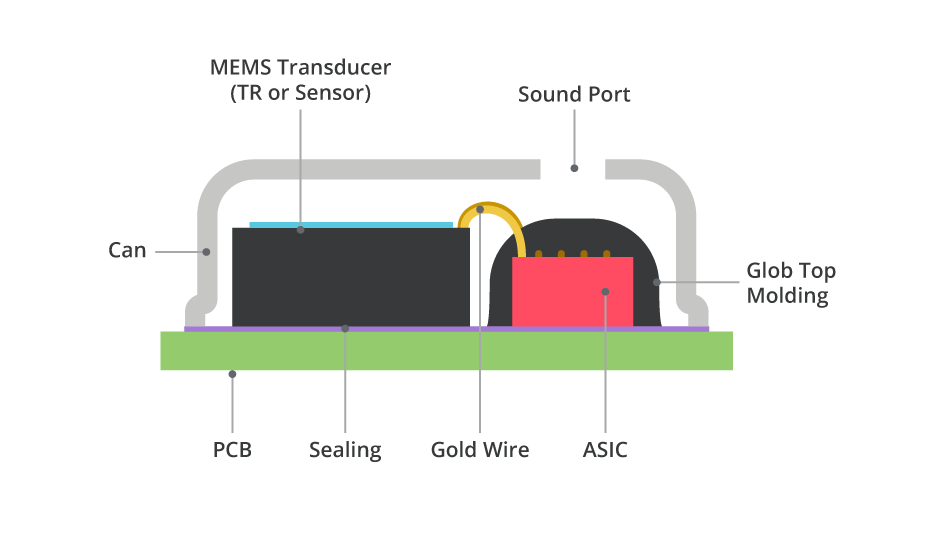
\includegraphics[width=8cm]{LiveAudioWatermarking/images/MEMS.png}
    \caption{: MEMS Structure}
    \label{fig:MEMS}
\end{figure}

\subsection{ECM}
An electret diaphragm (material with a fixed surface charge) is spaced close to a conductive plate, and similar to MEMS microphones, a capacitor is formed with the air gap as the dielectric. Voltage across the capacitor varies as the value of the capacitance changes due to sound pressure waves moving the electret diaphragm, $\Delta$V = Q/ $\Delta$C. The capacitor voltage variations are amplified and buffered by a JFET internal to the microphone housing. The JFET is typically configured in a common-source configuration, while an external load resistor and dc blocking capacitor are used in the external application circuit. \cite{mems}
\break
\begin{figure}[H]
    \centering
    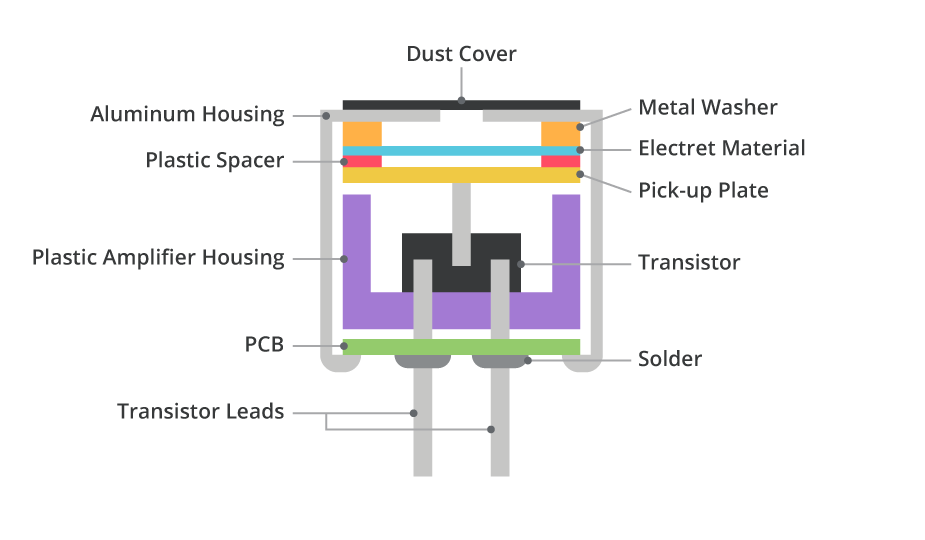
\includegraphics[width=8cm]{LiveAudioWatermarking/images/ECM.png}
    \caption{: ECM Structure}
    \label{fig:ECM}
\end{figure}
\section{Main differences}
Due to their small size, electrical noise immunity, and mechanical robustness, MEMS microphones are becoming increasingly popular. However, this does not mean that they are the de-facto best choice for every application. Many legacy applications may benefit from a simple change or upgrade to their current ECM. Apart from their excellent IP ratings, which allow them to perform well in harsh environments, the intrinsic nature of ECMs also makes them an excellent choice for applications that benefit from noise-canceling or unidirectionality.
\newpage
If the space constraints placed upon a design are particularly acute (such as in smartphones, wearables, hearing aid implants, etc.), or there is likely to be the need to distribute multiple microphones throughout an item of equipment (like in a VR headset for instance) then MEMS may be the better option.
Conversely, if elevated performance or resilience to challenging operating conditions are a priority, then ECM could prove to be the more appropriate route to take. Therefore, professional audio equipment, voice-controlled home assistants, voice recognition systems, and a wide range of other applications will continue to rely on these devices. \cite{compare}





 During the last decade the usage of MEMS in common devices raised significatively (back in 2009 when Apple started to use MEMS microphones for iPhone 4) and since the project focused on such devices like smartphones due to the nature of the attack and the target of the attacks, the solution that has been implemented was on MEMS microphones.
 As shown in Figure 1.3 it is possible to understand why it is much more useful for the purpose of this project to consider MEMS technology rather than the ECM, it is sufficient to consider Average Growth Rate to take into account the rising of the first technology and the falling of the latter.

 
 \begin{figure}[H]
    \centering
    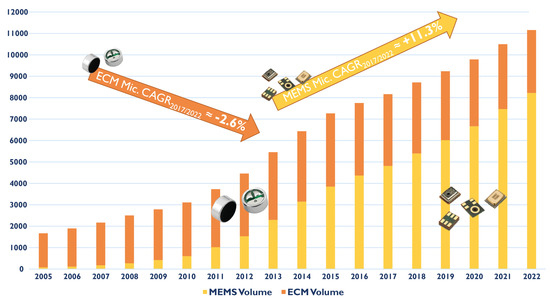
\includegraphics[width=10cm]{LiveAudioWatermarking/images/market.jpg}
    \caption{: Market Evolution}
    \label{fig:market}
\end{figure}

\section{Exploiting Non-Linearity in MEMS microphones}
Even though this effect is not exploited unless very high frequencies (order of 60kHz) are used it is really important to describe one of the core development of this project: the non-linearity of this technology.

Modules inside a microphone are mostly linear systems, in the case of the pre-amplifier with input S:
\[ S_{out} = A_1S\]
Acoustic amplifiers maintain a strong linearity only in the audible frequency range but outside of this range the response exhibits non linearity. Thus, for f $>$ 25kHz, the net recorded $S_{out}$ can be expressed as:
\[S_{out}\Bigg|_{f>25} = \sum_{i=1}^{\infty}A_iS^i=A_1S+A_2S^2+A_3S^3+...\]
With the third and higher terms that are extremely weak and can be ignored.

\newpage
To operate the microphone in its non-linear range, one can play a sound S composed of two tones S$_1$ = 40 and S$_2$ = 50 kHz.
S = $Sin(2\pi40t)+Sin(2\pi50t)$.
After passing through the diaphragm and pre-amplifier of the microphone, the output $S_{out}$ can be modeled as:
\[S_{out}= A_1(S_1 + S_2) + A_2(S_1 + S_2)^2 =\] \[ = A_1[Sin(\omega_1t) + Sin(\omega_2t)] + A_2 [Sin^2(\omega_1t) + Sin^2(\omega_2t) + 2Sin(\omega_1t)Sin(\omega_2t)\]
where $\omega_1$ = 2$\pi$40 and $\omega_2$ = 2$\pi$50.



The first order terms produce frequencies out of the microphone's cutoff, the second order term  instead is a multiplication of signals, resulting in different frequencies for each component such as 2$\omega_1$, 2$\omega_2$, ($\omega_1$ - $\omega_2$) and ($\omega_1$ + $\omega_2$). Mathematically, 
\[ A_2(S_1 + S_2)^2 = 1 - \frac{1}{2}Cos(2\omega_1t) - \frac{1}{2}Cos(2\omega_2t) + Cos((\omega_1 - \omega_2)t) - Cos((\omega_1 + \omega_2)t)\]
With the cutoff frequency at 24kHz, every frequency gets filtered except for the $\omega_1 - \omega_2$ component, that results in a 10kHz tone, this allows a totally inaudible frequency to be recorded by the microphone.
This is the main concept that revolves around this project and some possible future implementations and improvements. \cite{backdoor}




The goal of the project proposed is to show how some high frequency tones can carry some data thanks to Watermarking, anyway if the data can be carried at such high frequency the future improvement can basically carry these information at an even higher frequency thanks to the implementation of an amplifier and work at inaudible frequencies.



 \begin{figure}[H]
    \centering
    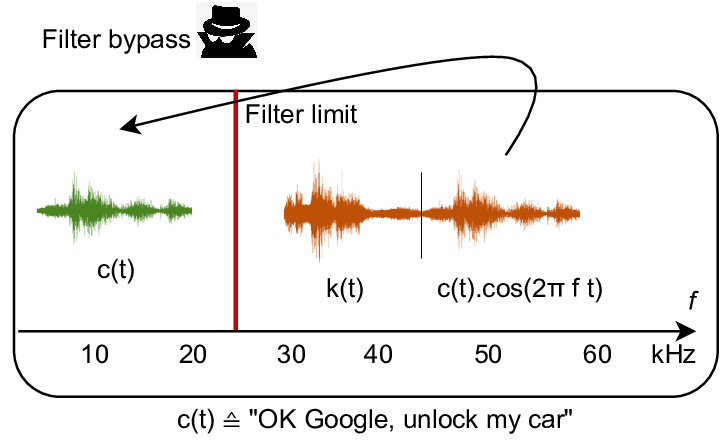
\includegraphics[width=10cm]{LiveAudioWatermarking/images/Bypass.png}
    \caption{: Example of a filter bypass exploiting non linearity}
    \label{fig:market}
\end{figure}
\setlength{\parindent}{0pt}
\setlength{\parskip}{2pt}
\chapter{Watermarking}
\section{Introduction to watermarking}
Watermarking is a technique used in both analog and digital works alike to embed \emph{usually} hidden information about the origin, the status or recipient of the host data. 

The core of the idea is to add a watermark signal to the data, in such a way that it cannot be easily detected by a standard user but can later be recovered from the mixed signal using the right key and algorithm. Since the watermark has to be concealed, its information is usually repeated all throughout the data with light modifications compared to the average amplitude of the original signal, so that it can always be recovered even if small amounts of watermarked data is available \cite[page 4, “Basic Watermarking Principles”]{hartung}.

A generic watermark signal usually depends on a key and the watermark information; sometimes it also depends on the data into which it is embedded. The extracted watermark, or relative confidence measure, instead is obtained using the watermarked data and the key, either in conjunction with the original data or not \cite[page 5, figs. 1-2, formulas 1-5]{hartung}.

Now, given the concept of a watermark, the needed qualities for a good watermark can be inferred \footnote{Note: all cited papers about watermarking had a dedicated section about requirements, Hartung \& Kutter however went more into detail. Some were deemed more important to list than others.} \cite[page 3, “Requirements”]{hartung} :
\begin{itemize}
	\item Robustness against standard manipulation: one of the major requirements. All manipulation and modification that the data might be subjected to throughout the distribution chain: conversions between different digital formats, digital to analog conversion, editing, printing. An attack in this context is every manipulation done with the purpose of rendering the watermark unrecognizable, destroying it or altering it.
	\item Imperceptibility: perceptual transparency, or the inability for the user to notice the watermark. The watermarking process should not introduce perceptible artifacts in the data. Nonetheless, it is desirable for a robust watermark's amplitude to be as high as possible, which is in direct contrast with the imperceptibility requirement. The implication is that a threshold must be found that does not cross the fine line of perception for the end user, but the subjectivity of human viewers/listeners makes it very difficult to find. Only they can be the final judges and tell if the presence of the watermark is compromising the fidelity of the original data or not.
	\item Density: a watermark should convey as much information as possible. Date of delivery, original recipient, source and every additional piece of information apt to find clues on the origin and use of the “incriminated” data. This is a soft requirement, because every use case has different demands. Some applications may need only to check if a watermark is present or not, while some others may need to embed large quantities of identifying data.
	\item Speed in embedding and retrieval: the algorithm should not be too complex or computationally expensive because real-time watermarking is a needed feature, especially in the case of live audio watermarking.
\end{itemize}

These qualities are what drives the development of different watermarking techniques, some of which will be better analysed and explained in the following chapters, focusing on the ones that have been found to be most useful within the scope of “live audio watermarking” but also giving a fast overview of other usages.

\section{Common use cases}
\subsection{As means of digital copy protection}

Watermarking is used on a wide variety of media, including text, video and audio. In this day and age the whole process, from creation and processing to distribution, is done digitally for all of the aforementioned media types. This provides many advantages, like transmission free of noise at a very cheap cost, ease of use through software and many more. Arguably, one the most important advantages of digital media is ease of reproduction without loss of fidelity. However, content providers do not find it a good quality, because it may hinder their ability to extract profits from their work. Mechanisms of digital copy protection are usually employed for this very reason (DRMs, or Digital Rights Management systems), but a paying user must have access to cleartext whom can then reproduce and illegally distribute copies. DRMs are usually successful in their purpose, at least for a starting period, but eventually always get circumvented. One last method for protecting IP rights is the insertion of a digital watermark into the data. Indeed its most frequent usage is copyright enforcement/protection. While it does not actively contrast illegal copying, it can be used at least as a last resort to identify source and destination of the multimedia data, allowing producers to engage in legal action if case should emerge \cite[page 1, “Introduction”]{hartung}.




Let us make an example for clarity's sake.
Let us imagine a producer that wants to do screening tests for their latest movie. They would need to send the product to untrusted parties that may leak it without the owner's approval. Even if they were trusted, a leak may always happen regardless (by means of hacking or lack of attention). How can a producer protect his or her work? One way would be to disincentivize sharing the protected work by threatening to cut ties, but this introduces the problem of identifying who did actually leak the work. This is where watermarking comes into use. A hidden piece of data, different for every subject whose work is sent to, is introduced into the movie itself. It is difficult if not impossible to notice but also robust to modifications. After obtaining the leaked data, an algorithm is used by the producing party to extract the watermark and identify who leaked the data. 


This is of course not the only use case. 

\subsection{As an authentication method}


Specifically, it is of interest the ability of a watermark to authenticate a recording.



A typical scenario is composed of a recording device and the people to be recorded (whether knowingly or not). The recording may be presented before a court of law and the person speaking may claim that the recording has been forged and so it is not valid as evidence. This puts the people that have the burden of proof in a difficult position because proving that an audio is forged is easy (audio tampering is easily spotted by looking at sudden cuts, differences in spectral signatures in different parts of the audio and abnormal peaks and valleys) but proving that it is not is really hard. In addition, in a court of law any alteration of the data after recording is considered tampering and consequently invalidating for evidence's purposes \cite[pp. 2-3, “Live audio watermarking for forensics”]{tictac}.

By embedding a watermark into a live recording (of a private conversation for example, but it may also be used in public speeches) there is a guarantee that if a malicious agent tries to modify it, they will modify the watermark too. In that case, the person talking can prove that recording is fake by extracting the watermark from the original recording and comparing it to the faked one, showing that they differ.



\setlength{\parindent}{0pt}
\setlength{\parskip}{2pt}

\chapter{Attack research} 


What follows is a series of brief descriptions of the watermarking techniques that have been found through research on various papers. Each paper is given a short introduction and a rapid overview on the method employed.



\section{BackDoor: Making Microphones Hear Inaudible Sounds}

Roy et al. \cite{backdoor} describe a method to introduce disturbances in the recording of an audio signal in such a way that they cannot be heard by human beings, but do appear in the final data. 


Being composed of frequency ranges outside the human hearing capabilities, a sound is designed specifically to exploit the non-linearities of the recording equipment, microphones found mainly in smartphones and IoT devices, so that a “shadow” sound appears in the audible range of the recording. 
Considering that this signal can be modulated, this enables the creation of a communication channel that can be used to transmit arbitrary data, on the order of 4kbps reported by the paper in certain conditions.



The idea of exploiting non-linearities in the recording equipment and of using ultrasonic signals for the live watermarking implementation has been inspired by this paper.


\section{Tic-Tac, forgery time has run-up! Live acoustic watermarking for integrity check in forensic applications}
Niță \& Ciobanu \cite{tictac} propose an interesting solution for the live audio watermarking problem. Their solution consists in the usage of a loud and recognizable sound, the ticking of a clock, to convey covert information. This brings a few advantages to usual watermarking methods:
\begin{itemize}
	\item It is a sound ubiquitous in its presence all throughout the world, meaning that even if it is loud it does not bring disturbance to the people listening because it is familiar.
	\item Being impulse-like in nature, the bandwidth of its signal is wide, making it very hard to be extracted from a recording and reused in another one to make it seem original.
\end{itemize}
The Tic-Tac signal, with a period of 1s, is injected in-between periods with small but imperceptible delays that can be modulated to an arbitrary message.

Another method for watermark injection is also provided due to the low SNR of the one mentioned above. It consists in generating a watermarking signal made by mixing a ticking sound with a chirp signal. A matched filter is obtained for the chirp signal as the decoding key. Finally, a modified clock positioned inside a room will broadcast an audio signal with a predetermined pattern that repeats every x seconds as long as a recording is taking place. Only an authorized person that knows the adapted filter will be able to extract the watermark.



\section{Robust audio watermarking in the time domain}
Bassia and Pitas \cite{robust} in Robust audio watermarking employ a simple method for watermark injection into audio data. However only on the digital side, namely MPEG Layer III and II files. 

The scheme proposed in the paper acts on the individual samples contained in the audio files, represented on either 16 or 8 bits, by changing the least significant bit of each one. The change is small enough in amplitude that it does not produce any perceptual difference. The key is the sequence of bits, which is randomly generated. 

The detector does not use the original signal and provides a confidence measure normalized between 0 (no watermark detected) and 1 (fully detected watermark). 

This method is solid enough to resist MPEG compression and both moving average and low pass filtering, with a worst case detection success of 99.8\%.


\section{Sonic watermarking}
Ryuki Tachibana \cite{sonichu} describes a method based on frequency subdivision of the original signal with a multi-bit message embedded into it together with a synchronization signal. 

The method is explained as follows. A sequence of power spectrums, calculated using short-term DFTs, is put together as a segmented area in a time-frequency plane called pattern block. Each pattern block is divided into tiles and the tiles in a row are called a sub-band. A pseudorandom number is used to assign values +1 and -1 to tiles and indicates their change in magnitudes. This pseudorandom number is the key given to the embedder and the detector.


The detection is performed by computing the magnitudes of the content for all the tiles, which in turn get correlated with the pseudorandom array used as a key.


The paper shows that this method is fast enough to compute to be used for live watermarking applications. Specifically, the paper tests different scenarios involving playing of solo, orchestral and popular music. The results showed very high detection rates for popular and orchestral music but acted very poorly on instrumental solos, because 
they often presented long intervals of silence. This implies preferred usage to be live shows and concerts, leaving speeches to other methods.



\chapter{Implementation Overview}
\section{Goal of the project}
The goal of this project is to implement an inaudible live audio watermarking solution that makes it possible to authenticate a live recording, enabling a person to speak and simultaneously guarantee that a recording of their speech will not be either forged or altered. 

The scope of the project is limited to recording devices that are available to most people, namely cheap and widespread ones: microphones embedded into smartphones, laptops, IoT devices and the like.


\section{Issues to be solved}
During the planning phase of the project, many issues surfaced on how to implement a solution with the required characteristics. % 



First and foremost, emphasis was put on providing a solution that would be easy to use and immediately available to end users. The choice fell on a smartphone app that could be readily downloaded from app stores \footnote{Since our project delivers a Proof of Concept, the app is distributed as an \emph{apk} file for Android smartphones only.}.



After that, the question has been posed of which data to transmit that might be useful for authenticity, but especially \emph{which} data to transmit, even though the proposed solution enables transmission of arbitrary packets of data (within limits). The application provides an easy way to embed GPS coordinates into the watermark, but the user is encouraged to include highly identifying info like e-mail addresses and ID numbers.




In chapter 2 the desirable qualities of a watermark have been addressed. Of those, it is indispensable for the watermark to be inaudible. The  solution had to take into consideration a transmission method that would not affect the quality of the recording, ideally to not be perceivable at all.

 
This has been a highly limiting factor for the choice of the frequencies (for the chosen method employs frequency manipulation) in which to transmit the watermark data, together with the sampling rate of the voice recording equipment and the tendency for microphones and recording software to be tuned to the low-frequency bandwidth \footnote{Frequencies in the audible range go from a minimum of 20Hz to a maximum of 20kHz, depending on sex and age.}. 


The suggested solution will be explained in further detail in the next section.




\section{Solution overview}
The implemented solution is split in two parts. 



The first is the provided application, intended to be used the most and by frequent (such as people active in PR) and occasional users alike. It is developed in such a way to be reasonably configurable, portable by means of being installable on every smartphone and tuned for the average user. The message inside the watermark, whether to encrypt it or not, options for the frequency, inclusion of the GPS coordinates: every one of these can be changed inside the app in a dedicated menu. 




The other half of the solution is a set of two tools to be used in conjunction that constitute the post-processing analysis capacity to check for the presence of a watermark inside a recording and, possibly, to extract the data hidden inside it. A MATLAB LiveScript for data detection and extraction and a CLI tool written in Kotlin that enables the MATLAB script, provided with the corresponding key, to decrypt the incoming string of bits.


An in-depth description of the solution, with its implementation details is presented in the next chapter.


\chapter{Implementation Details}
In this chapter is present a description of the implementation of the project, motivating the design choices.
% In this chapter is present a description of the implementation of the project, motivating the design choices.
\section{Preliminary evaluation of the target devices}
As previously mentioned, the target of this work are the most common available recorders nowadays: smartphones. Notably, Samsung and Apple smartphones, owing to their widespread usage, have been evaluated for the project purpose. Specifically, the analysis
focused on the audio signal captured by the default recording app on each device. Additionally, an Asus Windows PC was included in the evaluation process. 
To evaluate the feasibility of the watermark, an initial analysis of the frequency response of the recording system is needed. Firstly, the analysis has been conducted by recording audio samples from the smartphone devices, inside a regular room, without a specific noise, or sound.  The power density spectrum of a not-marked recorded samples is depicted in figure\ref{fig:FR}. In all the three cases the examined file is a MPEG-4 file (.m4a extension), with a sampling frequency $Fs = 44100 Hz$, therefore the resulting hypothetical watermarking signal cannot exceed the limiting maximum frequency of about $22 kHz$.
The spectrum is extracted using Matlab's Audio Toolbox Spectrum Analyzer\footnote{The spectrum can be seen by opening Matlab "Audio Test Bench" App, setting the file reader as input, clicking the button "Spectrum Analyzer" and then running the simulation.}. 

\begin{figure}[h]
    \centering
    \begin{subfigure}{0.48\textwidth}
  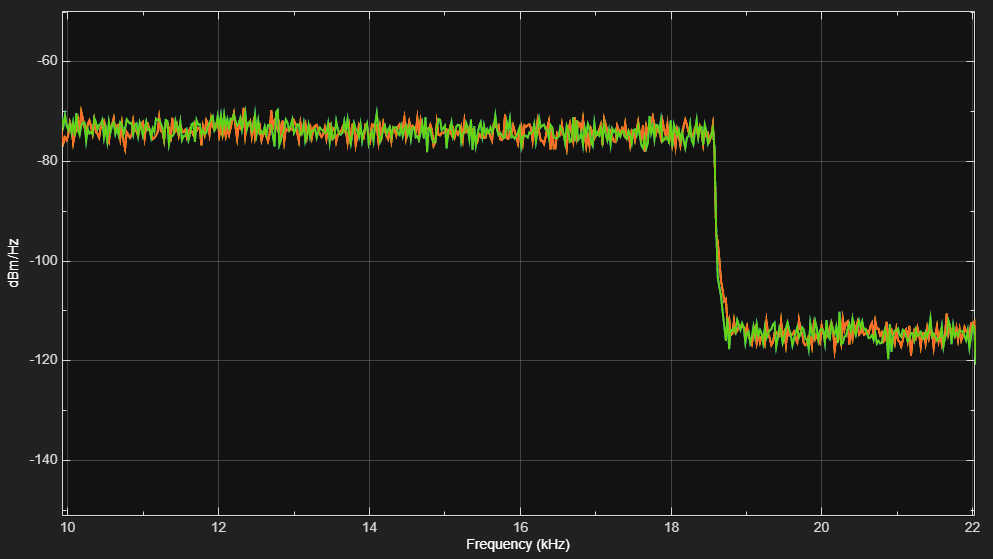
\includegraphics[width = \linewidth]{LiveAudioWatermarking/images/FRwindowsAsus.png}
    \caption{Density power spectrum of the signal recorded from Asus X507UF}
    \label{fig:FRwindows}
    \end{subfigure}
    \hfill
     \begin{subfigure}{0.48\textwidth}
      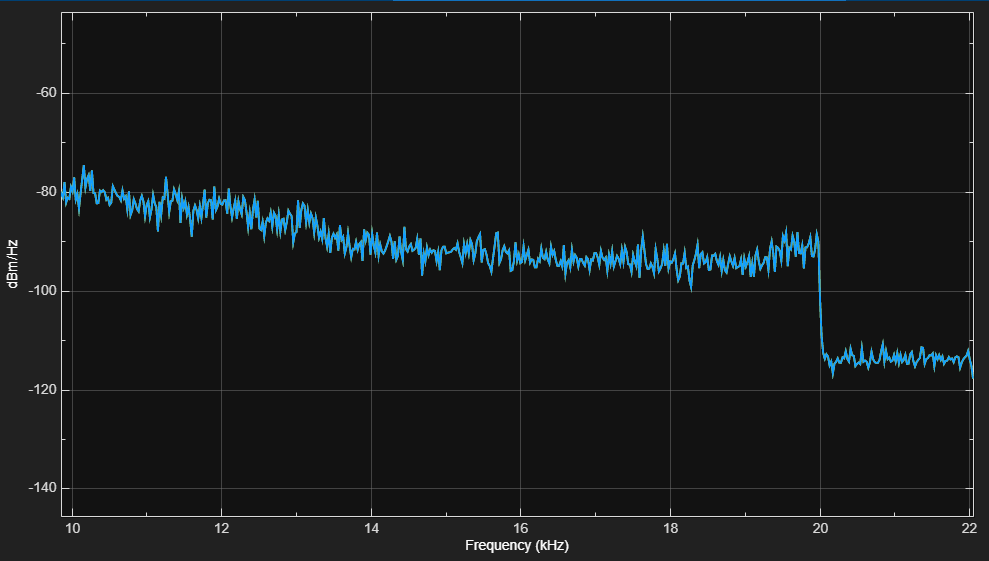
\includegraphics[width = \linewidth]{LiveAudioWatermarking/images/FRsamsung.png}
    \caption{Density power spectrum of the signal recorded from Galaxy Tab S6 Lite}
    \label{fig:FRsamsung}
    \end{subfigure}%
    \hfill
     \begin{subfigure}{0.48\textwidth}
    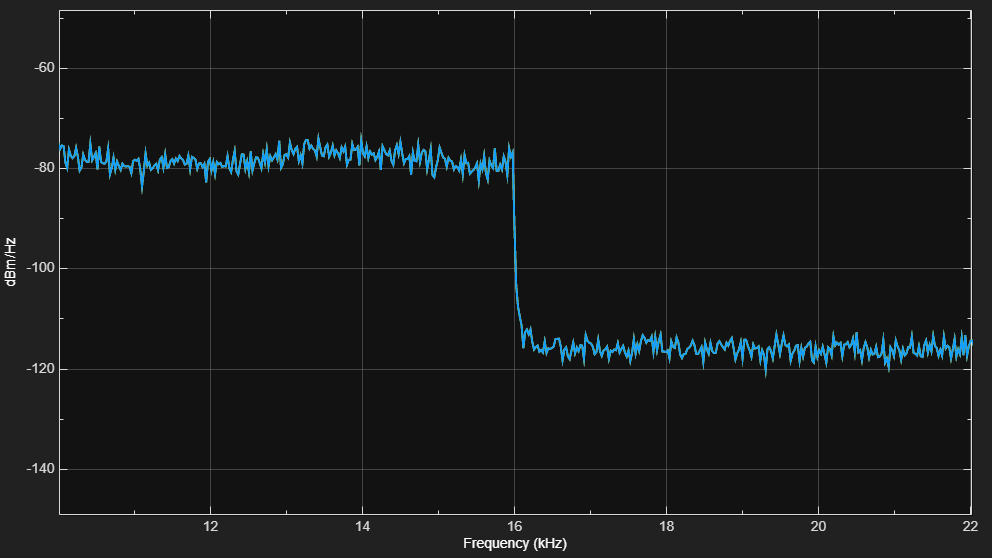
\includegraphics[width = \linewidth]{LiveAudioWatermarking/images/FRiphone14.png}
    \caption{Density power spectrum of the signal recorded from Iphone 14}
    \label{fig:FRiphone}
    \end{subfigure}%
    \caption{Frequency analysis of the signals}
    \label{fig:FR}
\end{figure}


From the results, it can be inferred that a low-pass filter is applied to the audio data, indeed the frequency response shows a the steep reduction at a certain frequency: 16kHz for iPhone, 19kHz for windows and 20kHz for Samsung. The attenuation at high frequency, in this case, may stem from both the hardware itself and the software used for recording. 
As an additional test, the response to a generated signal\footnote{The signal was generated using an \href{https://play.google.com/store/apps/details?id=com.keuwl.functiongenerator&hl=en}{Android application} on a Samsung s20+ 5G. The application's operation was validated using the computer's microphone as the input source, in "Spectrum Analyzer".} was analyzed, varying the frequency starting from 22 kHz and descending until the signal was clearly audible. The test confirmed that signals with frequency above the previously mentioned ones, are not detected, even at minimum distance and high intensity.

As a premise, it must been said that most adults have a hearing range below the 16kHz, but this value could change with respect to age (the lower the age the higher the frequency) and gender. This facts were proven by doing interviews, even though to a limited number of people. On average the best inaudibility results were obtained with frequency higher than 18 kHz, even if the generated tone remains audible to young female subjects. 

Consequently, considering watermark signal frequencies above this threshold results unfeasible with the apple products, while there is still some usable design range in Samsung's and Windows' devices.

\section{Implementation of the channel of transmission}
Considering the analysis performed by Roy et al.  \cite[page 5, BackDoor: Making Microphones Hear Inaudible Sounds]{backdoor} the solution for creating a communication channel consist in a FM modulated transmission. 
Differently from the paper approach, it is out of the scope of this project to result in a final frequency lower than the previously discussed range (e.g. 10 kHz), because it would lead to a perceivable sound in the final recording and therefore in a audible watermark. 
The channel used in this work is the data embedded in the recording with signals of which frequencies are greater or equal than 18 kHz, in order to occupy the higher end of the available spectrum.

\subsection{Evaluation of the method for transmitting data}
Digital data can be encoded and transmitted with different types of frequency modulation techniques, among the most common we selected ASK (Amplitude Shift Keying) and FSK (Frequency Shift Keying).
In FSK the frequency of the signal can assume two values: $f_{1}$ for transmitting bit '1' and $f_{0}$ for transmitting bit '0'. The binary data is therefore transmitted by means of a sine wave, which change frequency accordingly, as illustrated in figure \ref{fig:FSKbuild} 
\begin{figure}[h]
    \centering
    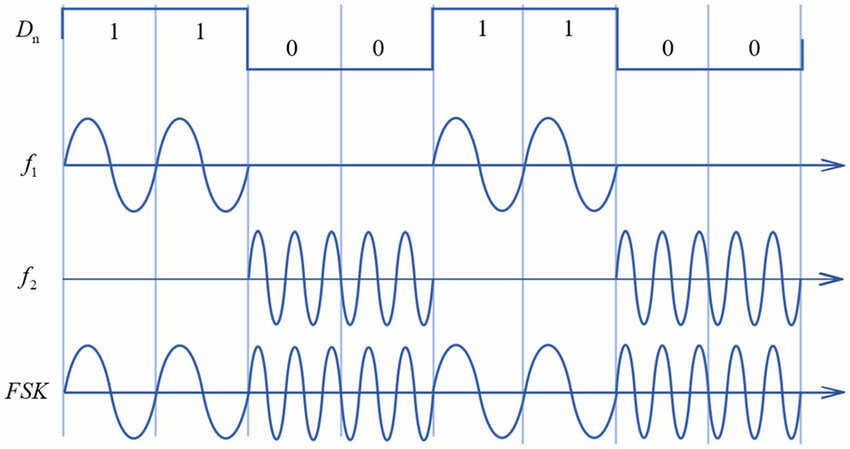
\includegraphics[width=0.8\textwidth]{LiveAudioWatermarking/images/FSK-modulation-wave-forms-example.png}
    \caption{Visual representation of the construction of an FSK modulated signal}
    \label{fig:FSKbuild}
\end{figure}

The FSK modulation can be easily transformed into a binary type of ASK, OOK (On-Off Keying), by setting one of the two frequencies at 0 Hz.
To easily detect the start and end of the transmission, two additional symbols (other than bit0 and bit1) have been added to the alphabet, therefore in a specific time interval the transmitted tone can assume 4 different frequencies ( $f_0, f_1, f_{start}$ and $ f_{stop}$). An example frame of one of the possible transmission of the character 'b' is shown in figure \ref{fig:FSK example}, from left to right represented symbols are bit start, bit0, 2 times bit1, 3 times bit0, bit1, bit0 and finally bit stop.

\begin{figure}
    \centering
    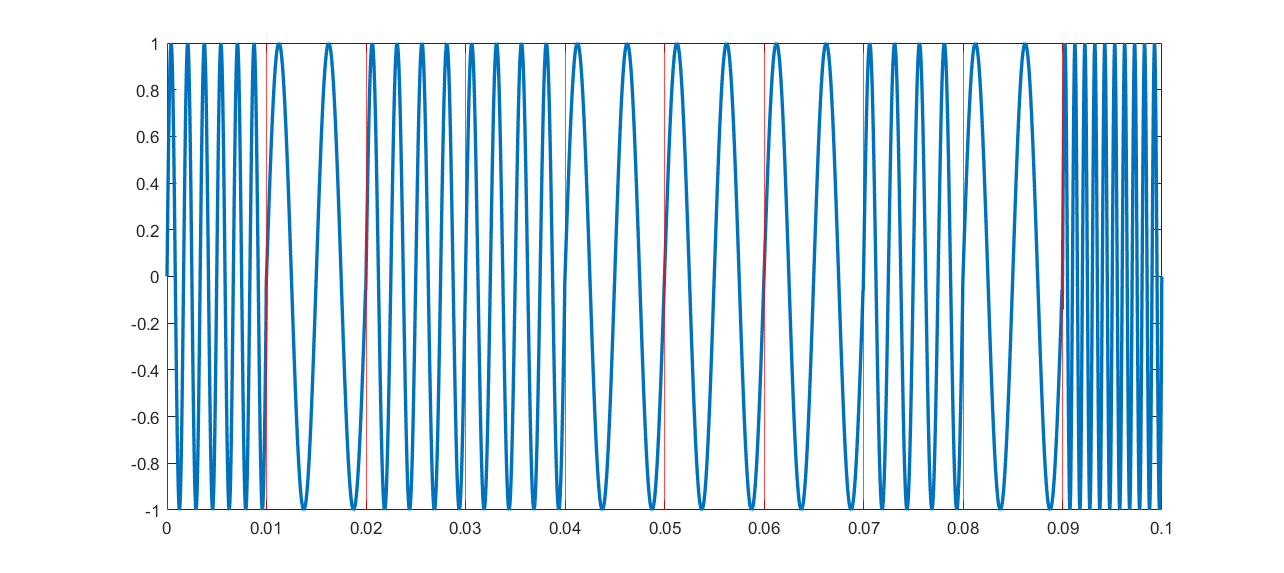
\includegraphics[width=\linewidth]{LiveAudioWatermarking/images/FSKex.png}
    \caption{Example of transmitted signal for a message composed of the character 'b'}
    \label{fig:FSK example}
\end{figure}

\subsection{Implementation of the platform used for transmitting the signal}
As previously discussed the most accessible way to use the watermark transmitter is by utilizing a smartphone app. For this purpose we developed a simple prototype application, in which the user can set the data and the parameters of the transmission. Moreover, since the application is installed on the user's smartphone, they can choose to embed meaningful information such as a real-time GPS position into the watermarking signal. The user is also able to set an encryption key that is then used to encrypt all the data to integrate in the signal through an “AES-256” algorithm, applied in Cipher Feedback Block mode, without Padding in order to keep the watermark track as short as possible. This mode can provide an additional protection against the modification of the audio sample, since, ideally, changing the order of the bits results in a message different from the transmitted one.
The application has been developed in Kotlin language, with Android Studio IDE.
The application is composed of two views: the home page and the settings.
\begin{figure}
    \centering
    \begin{subfigure}{0.30\textwidth}
        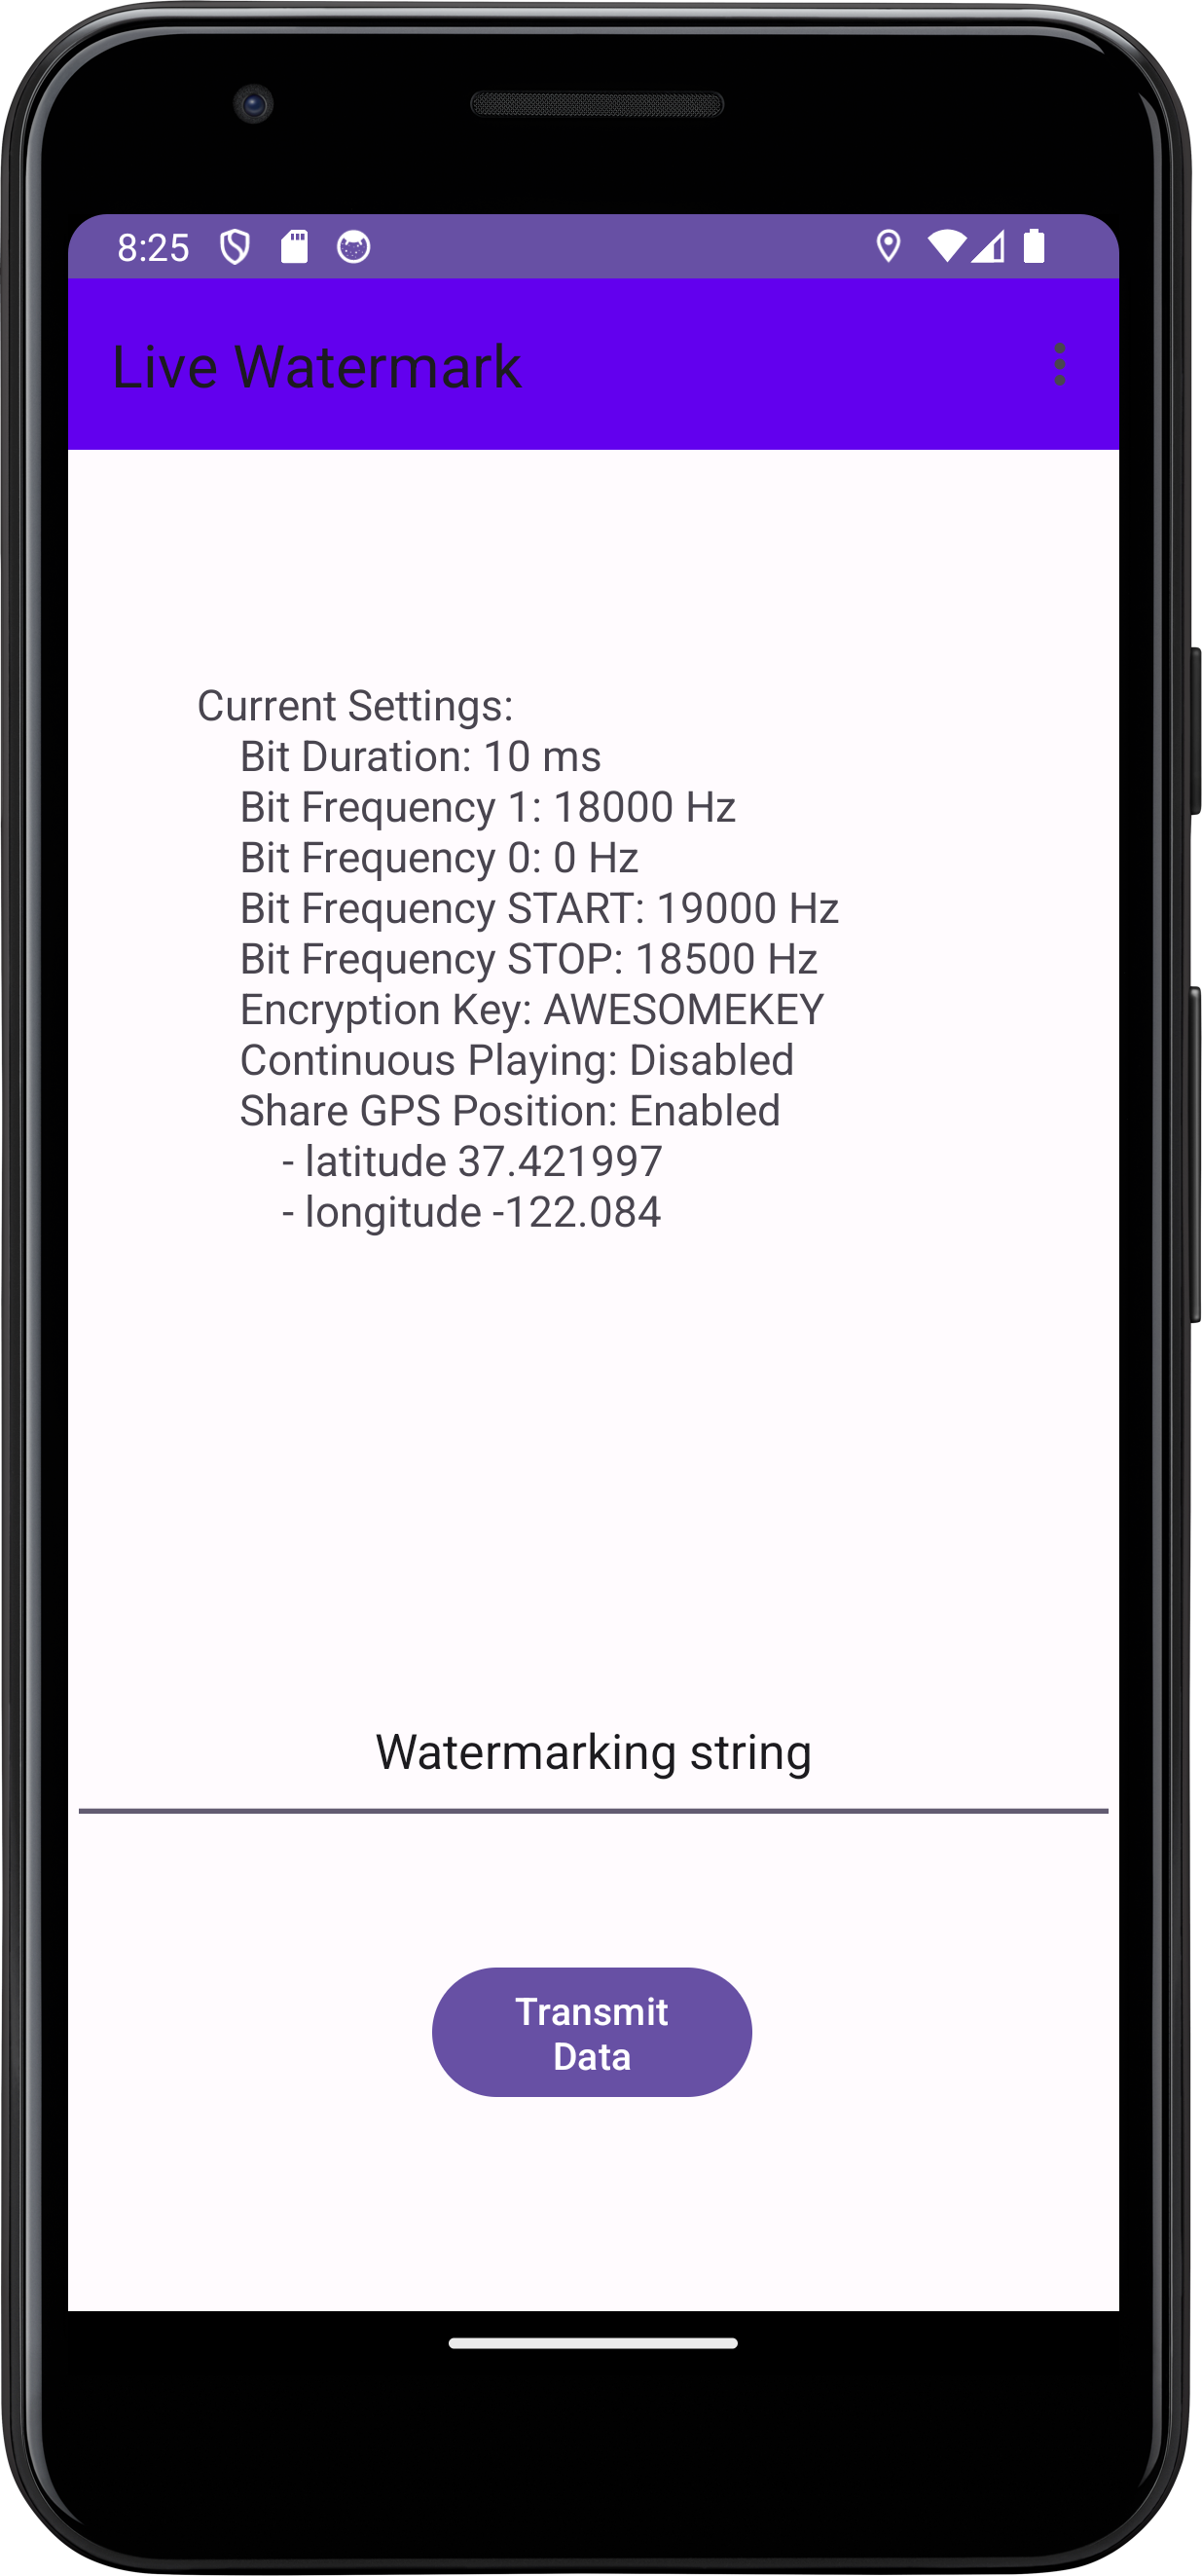
\includegraphics[width=\linewidth]{LiveAudioWatermarking/images/home_frame.png}
    \end{subfigure}
    \begin{subfigure}{0.30\textwidth}
        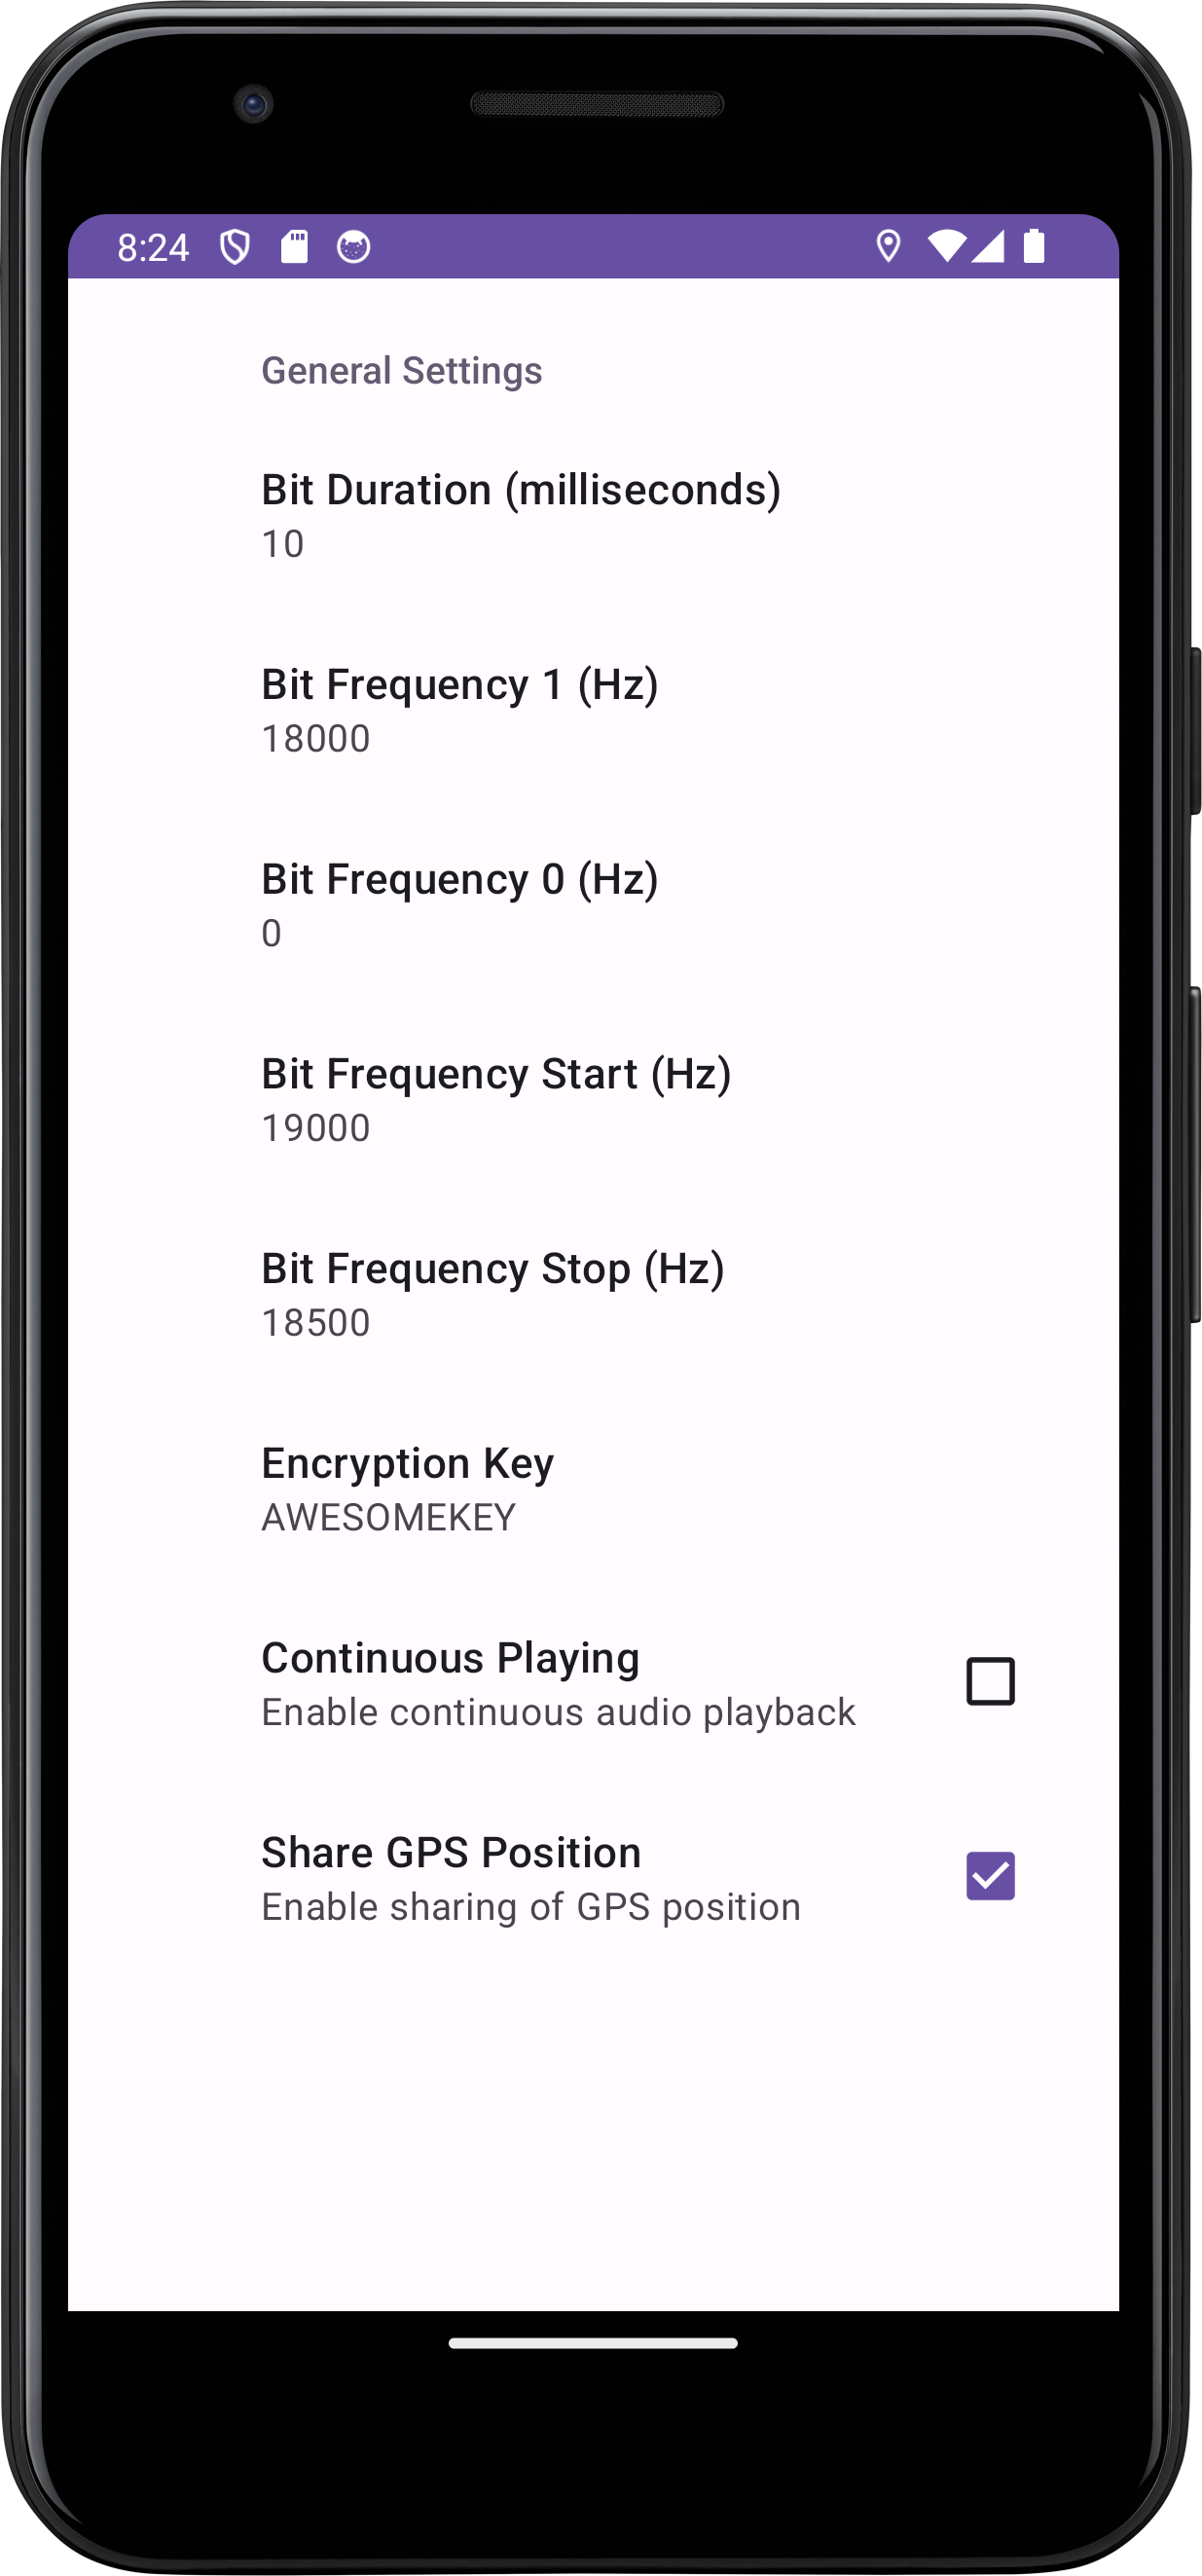
\includegraphics[width=\linewidth]{LiveAudioWatermarking/images/setting_frame.png}
    \end{subfigure}
    \caption{Main and Settings view of the application.}
    \label{fig:APP}
\end{figure}

From the main view the user can insert a string to use as a watermark. The transmission begins on pressing the "Transmit Data" button. In this prototype, there are no constraints on the format of the string or limitations on its size, except for the defaults set by the 'TextBox' object used.
In the Settings view the user can change the timing parameters previously described. The following source code shows the implementation of the transmit function, the complete code can be found in Appendix \ref{code}

\begin{lstlisting}[language=Kotlin, caption=Code of the Transmit and encrypt Function.]        
    private fun transmitData(data: ByteArray) {
        val minBuff = AudioTrack.getMinBufferSize(
            44100,
            AudioFormat.CHANNEL_OUT_MONO,
            AudioFormat.ENCODING_PCM_16BIT
        )
        val audioTrack = AudioTrack(
            AudioManager.STREAM_MUSIC,
            44100,
            AudioFormat.CHANNEL_OUT_MONO,
            AudioFormat.ENCODING_PCM_16BIT,
            max((44100 * BIT_DURATION / 1000 * data.toString().length), minBuff),
            AudioTrack.MODE_STREAM
        )
        audioTrack.play()
        val bitData = dataToBits(data)
        val start = generateTone(FREQ_BIT_START, BIT_DURATION)
        val stop = generateTone(FREQ_BIT_STOP, BIT_DURATION)
        audioTrack.write(start, 0, start.size, AudioTrack.WRITE_BLOCKING)
        for (bit in bitData) {
            val tone = if (bit == '1') generateTone(FREQ_BIT_1, BIT_DURATION)
            else generateTone(FREQ_BIT_0, BIT_DURATION)
            audioTrack.write(tone, 0, tone.size, AudioTrack.WRITE_BLOCKING)
        }
        audioTrack.write(stop, 0, start.size, AudioTrack.WRITE_BLOCKING)
        handler.postDelayed({
            audioTrack.stop()
            audioTrack.release()
        }, 100 * BIT_DURATION.toLong()) //delay added to finish the transmission before stop
    }

 private fun encrypt(plaintext: ByteArray, input_key: String): ByteArray {

        val key: SecretKey = SecretKeySpec(input_key.padStart(32, '0').toByteArray(), "aes")

        val emptyArray = byteArrayOf(
            0x00,0x00,0x00,0x00,0x00,0x00,0x00,0x00,0x00,0x00,0x00,0x00,0x00,0x00,0x00,0x00
        )

        // set cipher and options
        val cipher = Cipher.getInstance("AES/CFB/NOPADDING")
        cipher.init(Cipher.ENCRYPT_MODE, key, IvParameterSpec(emptyArray))

        return cipher.doFinal(plaintext)
    }

    \end{lstlisting}
The code makes use of other implemented function:
\begin{itemize}
    \item \texttt{dataToBits}: is a function that generates the binary string of the data
    \item  \texttt{generateTone}: is the function responsible of generating the vector containing the value of the tone to write on the stramed audioTrack.
    \item \texttt{encrypt}\footnote{Not explicitly called by the function, but conditionally executed on \textit{data} argument before it is called.}: is the function that apply the encryption algorithm. In this simple prototype, the Initialization Vector is a string of zeros. To enhance uniqueness and unpredictability, alternative approaches can be adopted, such as incorporating additional data or a combination of different data points, such as the device serial number, IMEI or a timestamp.
\end{itemize}

\section{Post-processing of the signal to retrieve the data}
To simplify the post processing identification of the data, it has been considered OOK-like transmission, with default parameters $f_{1}=18 kHz$, $f_{start}=19 kHz$, $f_{stop}=18.5 kHz$ and $tone\_length = 10 ms$. 

The analysis on the Audio track has been pursued with the help of Matlab. In particular, to automate the process and show the details of the signal, a Matlab Live Script has been coded. The script can be found in Appendix \ref{code}.

Below, the steps and methods applied to extract the embedded data from the recorded audio file are described.

\begin{enumerate}
    \item \textbf{extraction of the audio data from the MPEG-4 file}\\
    The data is stored into a vector using the program function ''audioread'', which extracts both the audio data and the sampling frequency from the file.
    \item \textbf{preliminary frequency analysis to prove the existence of the watermarking data}\\
    The analysis is made by performing the fft function on the vector of signal's data and observing the magnitude at the previously mentioned frequencies. 
    \item \textbf{Extraction of the raw watermark signal} 
    The frequencies of interest are simply isolated through a band pass filter, exploiting Matlab's \textit{bandpass} function.
    
    \item \textbf{Frequency analysis with efficient DFT algorithm}\\
    The algorithm used is Goertzel algorithm, which is very efficient for detecting the presence of a particular frequency component in a signal. It is more computationally efficient than the Fast Fourier Transform (FFT) for detecting a single frequency component. The algorithm calculates the discrete Fourier transform (DFT) of a specific frequency directly, without the need to compute the entire spectrum as FFT does. It is often used in applications such as tone detection in telecommunications and audio processing. The resulting magnitudes are used to compute the thresholds used in the next step.
    
    \item \textbf{Derivation of the transmitted binary string} \\
    The segment of the vector containing the watermark is isolated and extracted by searching the start and stop bit. To search for the right index, a cross correlation with a generated bit start tone is computed, the index of the maximum in the resulting vector represent the delay at which the start(stop) tone is found. Knowing the positions of these bits, it is possible to compute the number of tones present in the sample. Consequently each one segment is analyzed with Goertzel algorithm and compared against the threshold, which consists of the previous threshold multiplied by a constant empirically defined.
    
    \item \textbf{Decryption and interpretation of the binary string}\\
    If the transmitted data is encrypted, it can be decrypted using the provided tool, whose decrypting function code is listed here, the full code can be found in Appendix \ref{code}.
\begin{lstlisting}[language=Kotlin]
    fun decrypt(ciphertext: ByteArray, input_key: String): ByteArray {

    // exactly same code as function "encrypt" but in decryption mode
    val key: SecretKey = SecretKeySpec(input_key.padStart(32, '0').toByteArray(), "aes")
    val iv = byteArrayOf(0x00, 0x00, 0x00, 0x00, 0x00, 0x00, 0x00, 0x00, 0x00, 0x00, 0x00, 0x00, 0x00, 0x00, 0x00, 0x00)
    val cipher = Cipher.getInstance("AES/CFB/NOPADDING")
    cipher.init(Cipher.DECRYPT_MODE, key, IvParameterSpec(iv))

    return cipher.doFinal(ciphertext)
}
\end{lstlisting}
The code use the same library and approach that can be found in the application code.

\end{enumerate}


Also a variant of the live script has been developed, it simply record some second of the input data and then performs the same analysis

%retriving the sample, isolating the freq of interest, apply goertzel algorithm to analyze the energy of the signal at each frequency and calculate the thresholds, searcing for start bit  and stop bit, calculating the number of simbols, divide the signals into intervals and then evaluating again the content of the interval compared to the thresholds


% This is where you explain what you have implemented and how you have implemented it. Place here all the details that you consider important, organize the chapter in sections and subsections to explain the development and your workflow.\\Given the self-explicative title of the chapter, readers usually skip it. This is ok, because this entire chapter is simply meant to describe the details of your work so that people that are very interested (such as people who have to evaluate your work or people who have to build something more complex starting from what you did) can fully understand what you developed or implemented.\\Don't worry about placing too many details in this chapter, the only essential thing is that you keep everything tidy, without mixing too much information (so make use of sections, subsections, lists, etc.). As usual, pictures are helpful.
\chapter{Results}
A watermarked audio sample has been recorded\footnote{The recording was made with Samsung Tab S6 Lite. The audio watermark, however, is emitted from a Samsung S20+ 5G.} and then analyzed with the script listed in Appendix \ref{code}. Here the results are reported and discussed.
\section{Analysis of the result of a watermarked audio recording.}
As a first step, let's analyze the spectrum and magnitude of the "raw" signal.
In figure \ref{fig:raw_signal} is reported the spectrum of the signal on the left (\ref{fftraw}) and the plain signal on the right (\ref{rawsig}). The audio sample comprises a sentence ("example of watermarked audio") that has been marked using the previously described application. The watermark is set to a simple string ('ciao') and a GPS location, both encrypted with the methods previously explained, using as key the string \textit{"AWESOMEKEY"}.
\begin{figure}[H]
    \centering
    \begin{subfigure}{0.48\textwidth}
    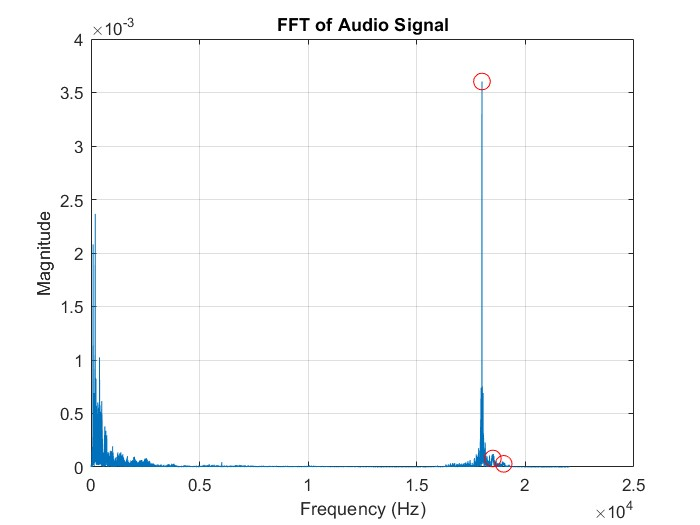
\includegraphics[width=\textwidth]{LiveAudioWatermarking/images/FFT_raw.jpg}
    \caption{}
    \label{fftraw}
    \end{subfigure}%
    \hfill
     \begin{subfigure}{0.48\textwidth}
    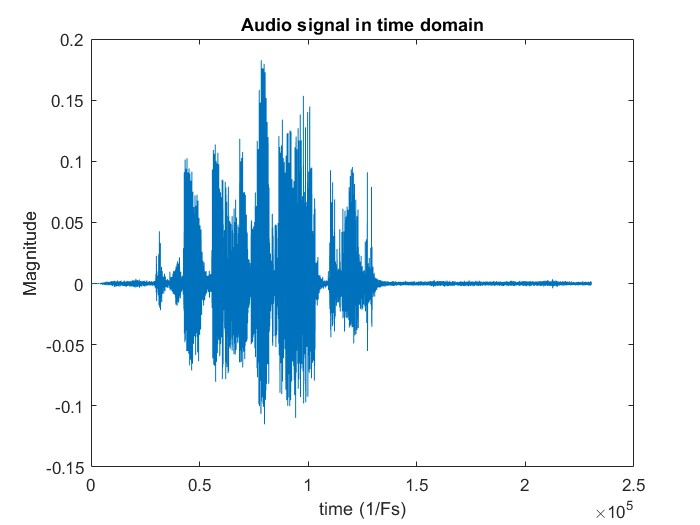
\includegraphics[width=\textwidth]{LiveAudioWatermarking/images/sig_td_raw.jpg}
    \caption{}
    \label{rawsig}
    \end{subfigure}
    \caption{Unprocessed audio sample}
    \label{fig:raw_signal}
\end{figure}
It can be observed from the figure that there is some content at the desired frequency, indicating that the watermark has been successfully embedded into the audio file.
The result of the applied band-pass filter is shown in figure \ref{fig:filtered_signal}. The filtered data contains only the audio watermark. When listening to the processed signal, no noise can be heard.


\begin{figure}[H]
    \centering
    \begin{subfigure}{0.48\textwidth}
    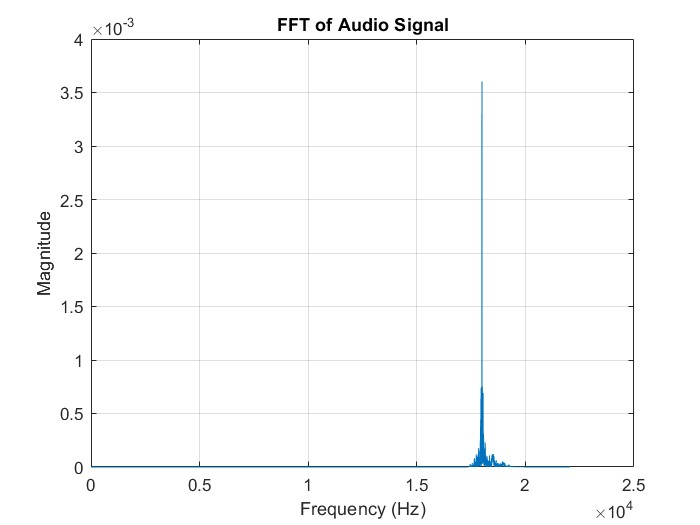
\includegraphics[width=\textwidth]{LiveAudioWatermarking/images/FFT_filtered.jpg}
    \caption{}
    \label{}
    \end{subfigure}%
    \hfill
     \begin{subfigure}{0.48\textwidth}
    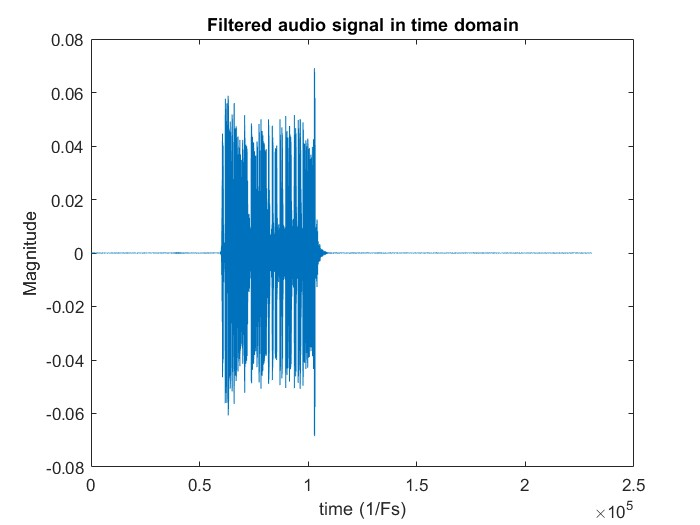
\includegraphics[width=\textwidth]{LiveAudioWatermarking/images/sign_td_filt.jpg}
    \caption{}
    \label{}
    \end{subfigure}
    \caption{pre-processed audio sample}
    \label{fig:filtered_signal}
\end{figure}

The subsequent phase involves determining the positions of both the start and stop bits. For this purpose, cross-correlation analysis was conducted using the 'xcorr' command in Matlab between a tone generated in the script and the pre-processed audio track. The results of these analyses are displayed in figure \ref{fig:tonesearch}. The red circle indicates the index (more precisely the \textit{lag} with respect the start of the audio sample) at which the tone begins.

\begin{figure}[H]
    \centering
    \begin{subfigure}{0.48\textwidth}
    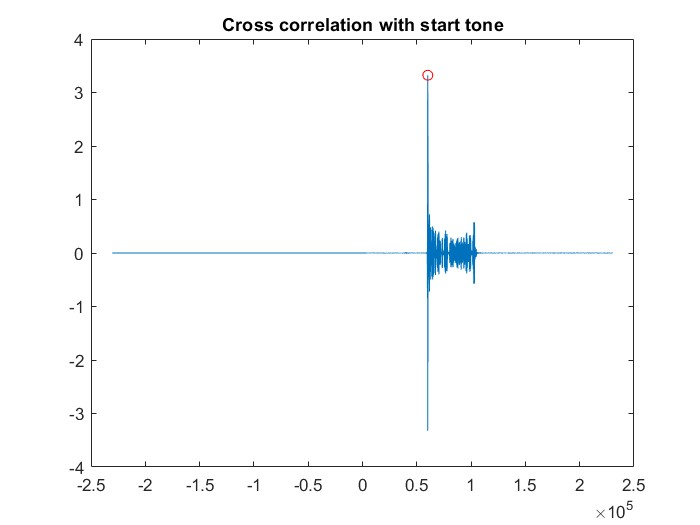
\includegraphics[width=\textwidth]{LiveAudioWatermarking/images/cross_start.jpg}
    \caption{}
    \label{}
    \end{subfigure}%
    \hfill
     \begin{subfigure}{0.48\textwidth}
    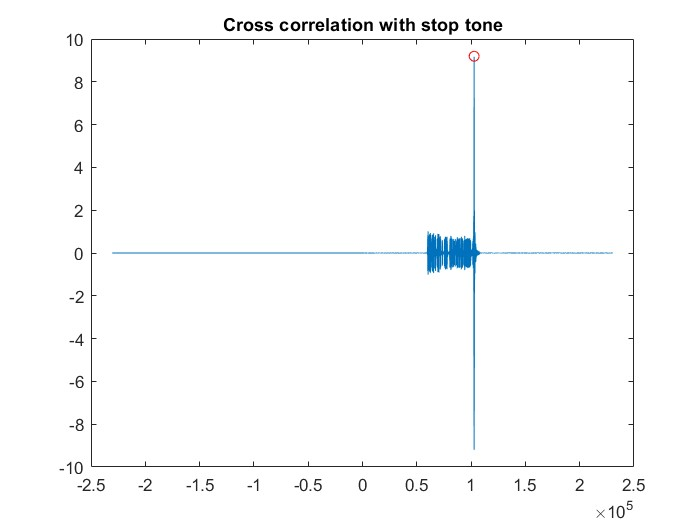
\includegraphics[width=\textwidth]{LiveAudioWatermarking/images/cross_stop.jpg}
    \caption{}
    \label{}
    \end{subfigure}
    \caption{cross correlation results}
    \label{fig:tonesearch}
\end{figure}

After identifying these tones, we can deduce the length of the watermark. By knowing the duration of the tone, we can extract segments for further analysis using additional signal processing techniques. a representation of the segments can be found in figure \ref{fig:segments}
\begin{figure}[H]
    \centering
    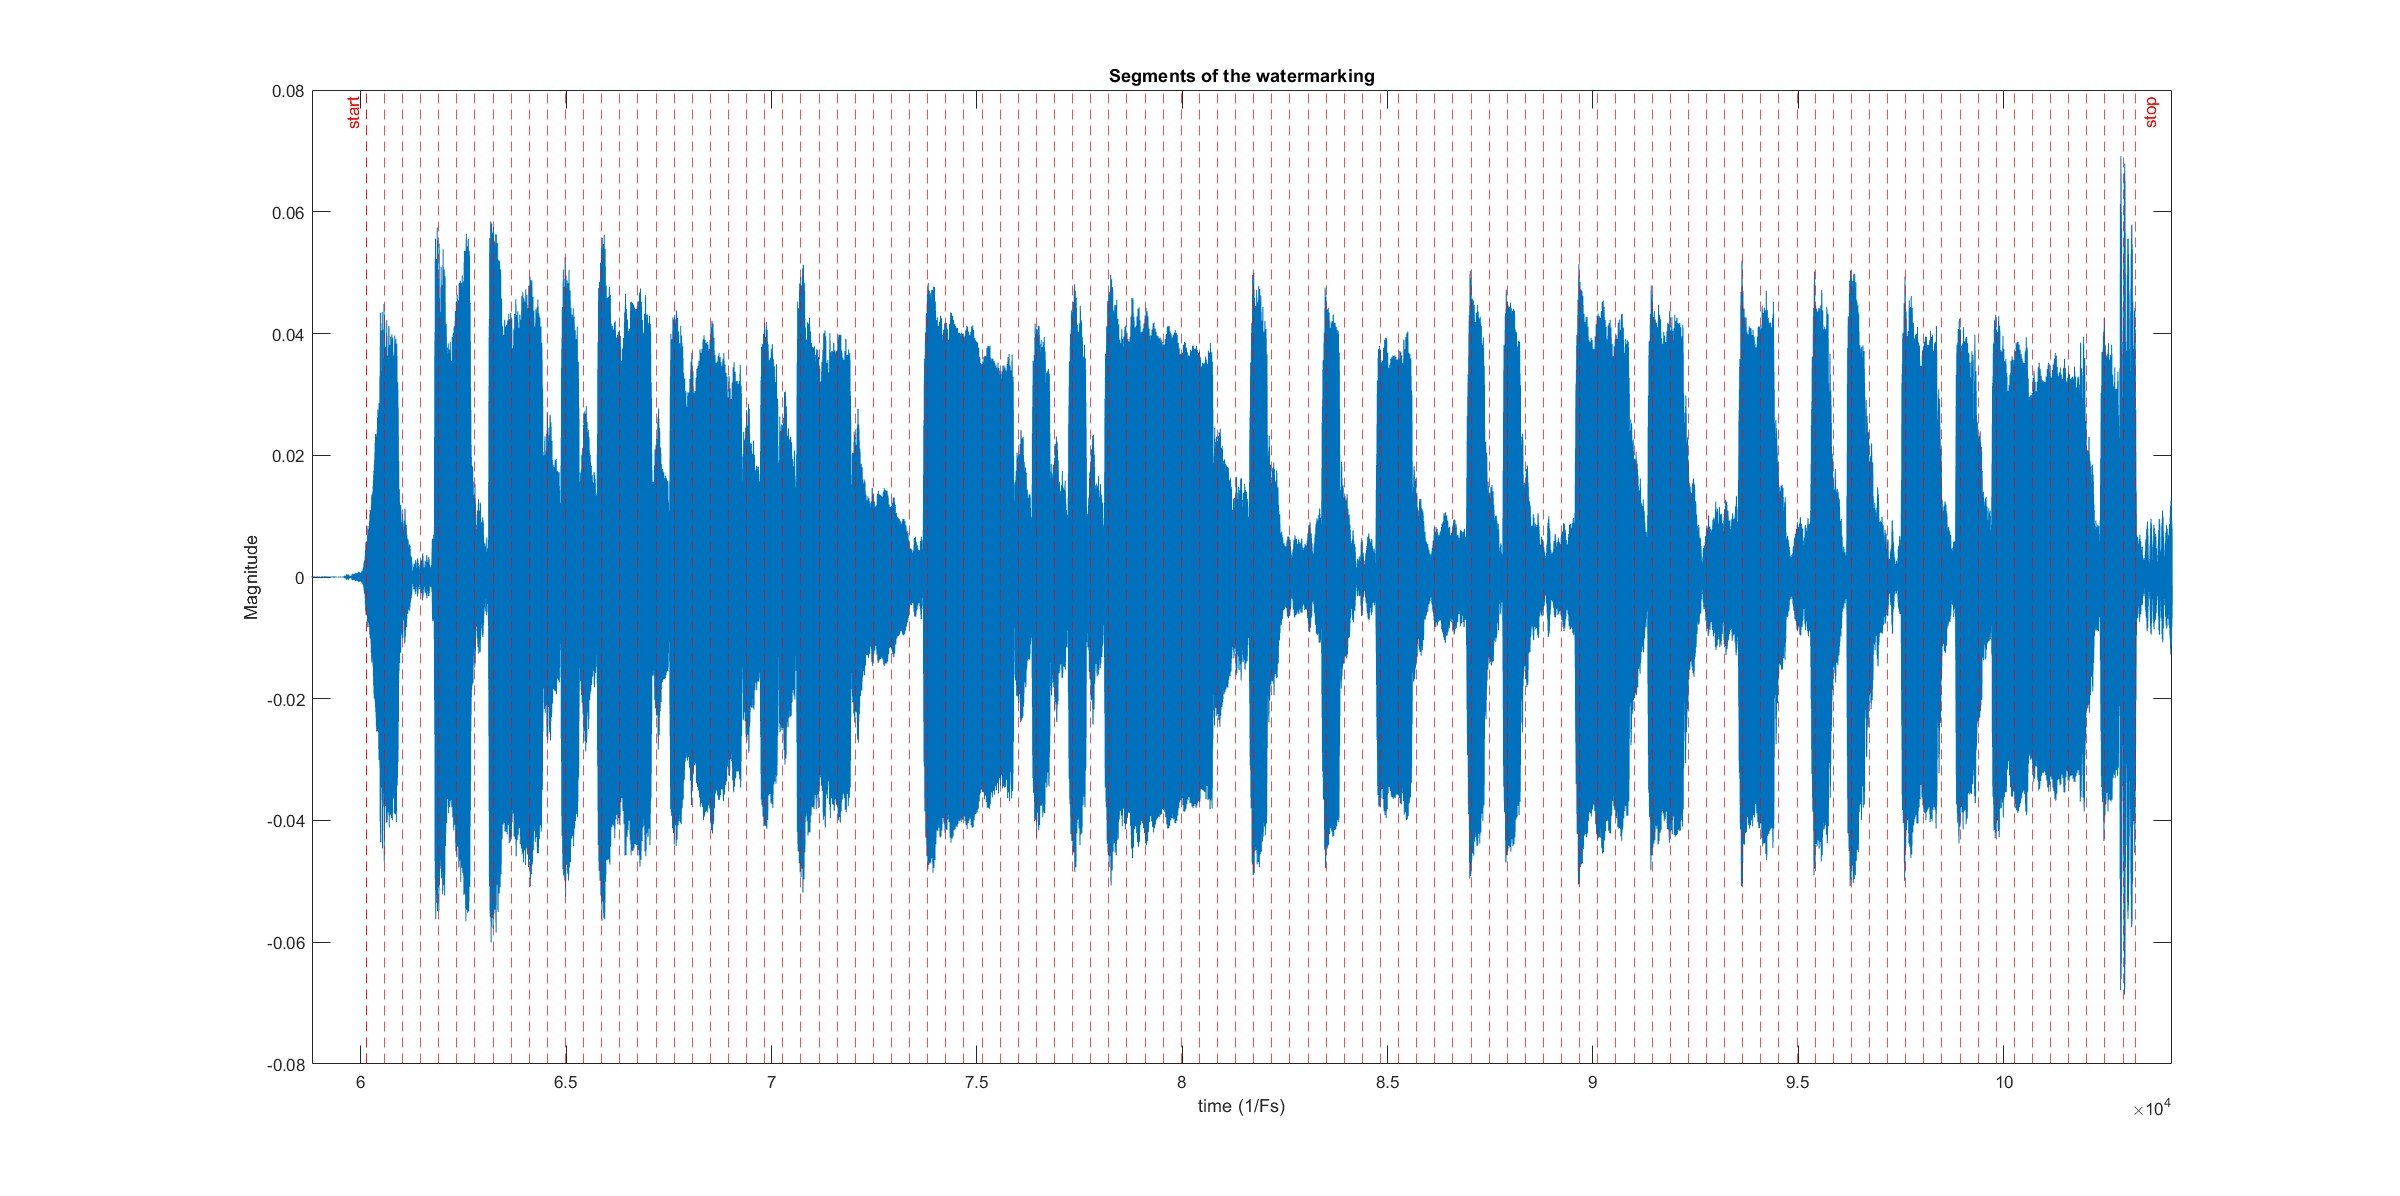
\includegraphics[width=\textwidth]{LiveAudioWatermarking/images/sgments.jpg}
    \caption{Segments representing the tones in the audio sample.}
    \label{fig:segments}
\end{figure}

Before assessing the segments, it is essential to establish a threshold that allows to determine whether a frequency (and consequently a symbol) is present within a segment or not. 
To accomplish this objective, an analysis with Goertzel algorithm is made, the result are showed in figure \ref{fig:goertzel}. 
\begin{figure}[H]
    \centering
    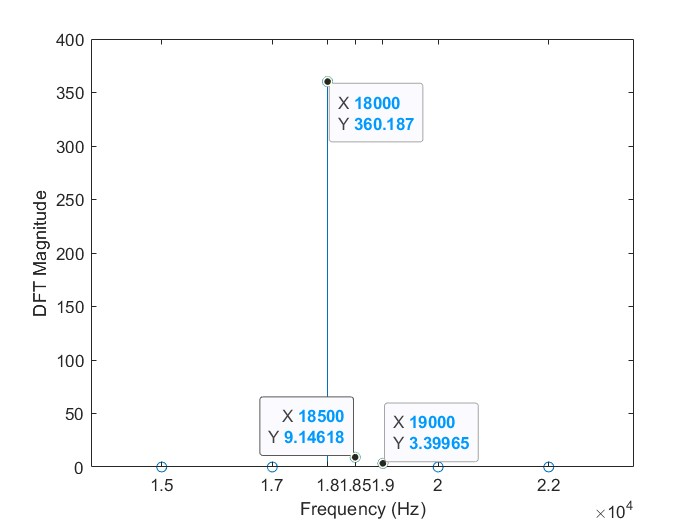
\includegraphics[width=0.8\linewidth]{LiveAudioWatermarking/images/Goertzel-full.jpg}
    \caption{Analysis with Goertzel Algorithm}
    \label{fig:goertzel}
\end{figure}

The values highlighted in the figures changes in every recording, therefore the needed threshold depends on the energy of the signal, that is not guaranteed to be constant throughout the sample (i.e. within a segment, one may find a magnitude different from that in another segment representing the same symbol).
A simplistic approach has been adopted: Assuming the frequency is distributed across all segments, one can calculate a sort of average energy by dividing the magnitude of the frequency in the entire signal by the total number of segments. This value can then be adjusted as needed (since each track is unique) by simply multiplying it by a constant.
In the context of this specific scenario, the number of segments has been computed. Consequently, the mean value is computed by dividing the overall signal magnitude by this quantity. 
\[Thr_{symb} = k\times\frac{ABS(goertzel(f_{symb}))}{N_{seg}}\]
In light of the aforementioned reasons the determination of \textit{k}, in this project,  is empirical, the attributed value is 0.8. For the start and stop bit, since the energy is cointained in a single segment, the chosen threshold is half of the total magnitude.
In figure \ref{fig:symbols} the results of the Goertzel algorithm applied to the segments are depicted. Specifically, an analysis per symbol is presented. From the represented values, the recognition mechanism of each one is easily discernible: each magnitude is compared to its threshold and the magnitudes of the other symbols, yielding the result readily.
\begin{figure}[H]
    \centering
    \begin{subfigure}{0.48\textwidth}
    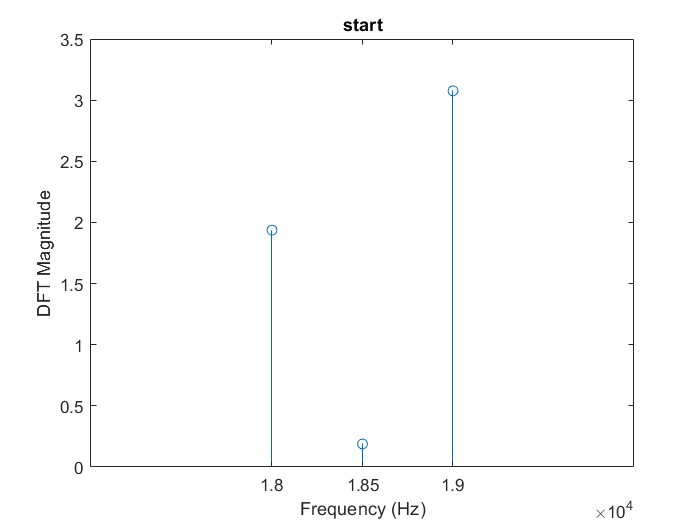
\includegraphics[width=\textwidth]{LiveAudioWatermarking/images/start_bit.jpg}
    \caption{}
    \label{}
    \end{subfigure}%
    \hfill
     \begin{subfigure}{0.48\textwidth}
    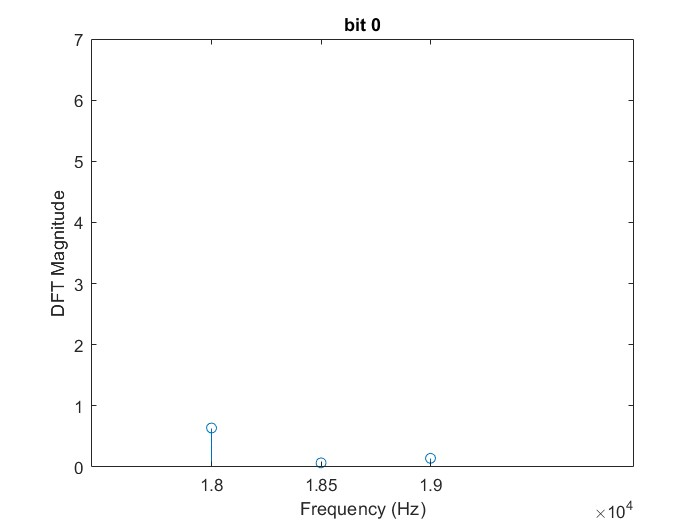
\includegraphics[width=\textwidth]{LiveAudioWatermarking/images/bit0.jpg}
    \caption{}
    \label{}
    \end{subfigure}\\
        \begin{subfigure}{0.48\textwidth}
    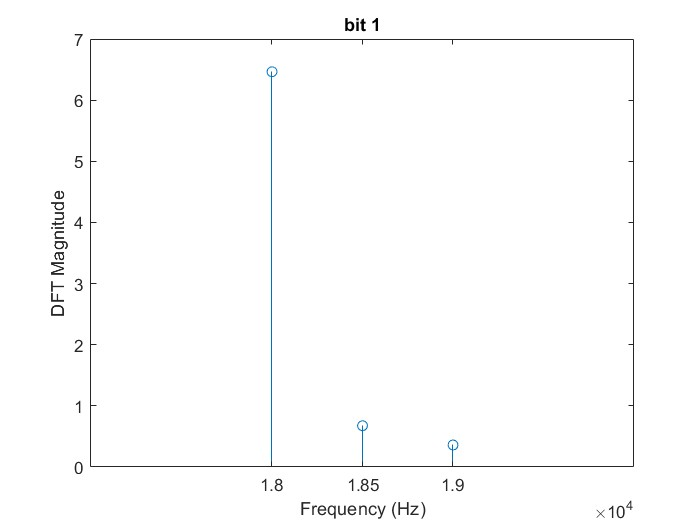
\includegraphics[width=\textwidth]{LiveAudioWatermarking/images/bit1.jpg}
    \caption{}
    \label{}
    \end{subfigure}%
    \hfill
     \begin{subfigure}{0.48\textwidth}
    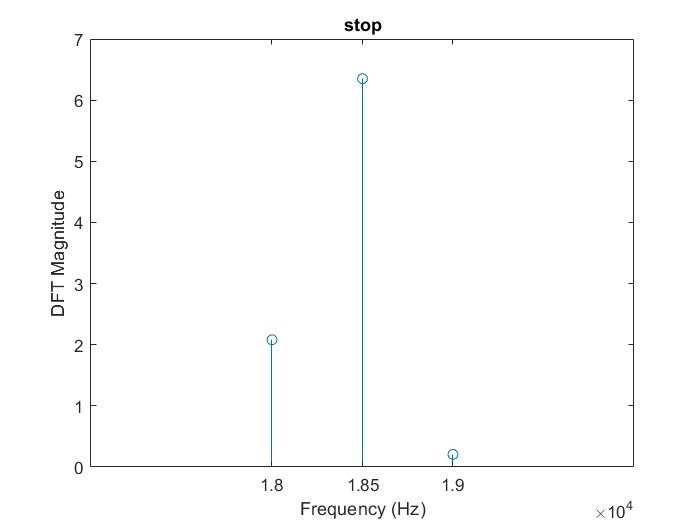
\includegraphics[width=\textwidth]{LiveAudioWatermarking/images/stop_bit.jpg}
    \caption{}
    \label{}
    \end{subfigure}
    \caption{Frequency encoding of the symbols}
    \label{fig:symbols}
\end{figure}
In this case the received binary string is "9BAEF5C3EAFE898A3B194D7D", that can be represented as a Unicode string, but the encrypted output manifests as a sequence of seemingly random characters, devoid of any meaning.
At this stage, the solution to retrieve the data, is to employ the designated decryption tool. The tool is invoked with Matlab's command \texttt{system()}, passing as arguments the binary string (in binary representation) and the previously defined encryption key, the output is saved in case further operation are needed.

In this experiment the resulting string still contains unintelligible characters: those are the latitude and longitude values of the GPS location, that needs to be converted into a IEEE 754 float representation.

Finally the watermark is successfully extracted and the information are in human readable form.

\section{Known Issues}
The work described in the preceding sections was conducted in a controlled environment, with the following characteristics:
\begin{itemize}
    \item \textbf{The room was not noisy}, even if the audible noise (e.g. air condition, chatter etc), does not have impact on the selected frequency and it is filtered.
    \item \textbf{The watermarking device was situated a few centimeters away from the microphone}, to guarantee a sufficient power to detect the signal
    \item  \textbf{The transmission was kept short}, since the watermark is extracted with simple signal processing technique
    \item  \textbf{The bitrate was set to an already verified value}, since the tone length was set to 10 ms the bitrate is 100 bit/s, that is sufficient considering recordings of a minimum duration of few seconds, but relatively slow considering the sampling frequency.
\end{itemize}

This characteristics stem from the issues encountered during the experimental trials, which are:
\begin{itemize}
    \item \textbf{Non-linearity of the smartphone's speaker:} when playing the audio watermark, sudden frequency shifts occurs. In an ideal case, this should not result in any noise coming from the device, but in this implementation,  a \textit{"crackling"} sound is audible. This sound is below the designed frequencies, indeed it is removed by the band pass filter. 
    At the current state of the project, the source of this issue is not totally certain but possible improvement are discussed in the \textit{Future Work} section.
    \item \textbf{Limiting range of near-ultrasound frequencies tones:} as previously discussed the implementation has been pursued with devices that are suitable for the selected frequency range, therefore the functionality is not guaranteed on other devices (e.g. Iphone). This issue affects also the recognition of tones with the cross correlation, since the tones have similar frequency.
    \item \textbf{Possible instability of the developed software:} the developed application is a prototype, therefore the performance and correctness of the code is not guaranteed: some delays have been noticed in long transmission (e.g. irregular tone duration) that can lead to misinterpretation of the symbols, because of misalignment of the symbol's window.
    Furthermore, with the current software, setting a lower duration of the tone may result in a tone skip, or no output at all.\\
    The output of the first tone has some latency, resulting in having a lower magnitude with respect to the others.
    The script for decoding the watermark may need \textit{"ad-hoc"} tuning for retrieving sample in some condition ( e.g. changing the threshold, failing to detect start/stop tone).

    
\end{itemize}

\section{Future Work}
%Adding a section about how to improve the project is not mandatory but it is useful to show that you actually understood the topics of the project and have ideas for improvements.%
Considering the issues listed in the previous section, we can outline some potential improvements to be addressed as future work. 
The first improvement consist into a better quality of the watermarked signal: starting from the software, an experience app developer or a more in depth research endeavor, can make application transmit a more sharper signal, solving the issues related to timing performances. Also, alternative approaches to the chosen modulation technique can improve both the density of the watermark and its robustness, for example APSK (Amplitude and phase-shift keying) allows for a lower bit error rate, at the cost of the increased complexity in the development of a transmitting e receiving software.
Regarding the hardware, utilizing an external device such as a mini speaker equipped with ultrasonic transducers, connected to the smartphone's audio interface (e.g., audio jack, Bluetooth, USB-C), could significantly enhance the signal. This external device has the capability to reproduce '0' and '1' bits at a higher frequency, ensuring superior performance and potentially amplified power. Additionally, the transmitted signal can be split into stereo channels, allocating the right channel for one bit symbol and the left channel for the other, further optimizing the transmission process. Furthermore, the ultrasonic transducers, being capable of working in ultrasound frequency, open up the possibility of injecting a signal into frequencies near ultrasound, leveraging the intrinsic nonlinearities of the MEMS microphones.

Another area of enhancement of this work is to developed a better post processing analysis, exploiting more complex and advanced technique used in modern digital signal processing.
An additional feature that can be developed is live processing, making the less experienced users able to easily check the presence of the watermark and its content.

Regarding the data to be embedded in the signal, there exists a plethora of possibilities. Unique device identification codes, such as IMEI numbers, can be retrieved. Additionally, a wide array of sensors available on any smartphone offers diverse choices for data incorporation.
\chapter{Conclusions}
To sum up the previous chapters and also give a brief recap it is possible to state that this project showed how watermarking and high frequency signals can be used to manipulate data.




This project, through the studying of the state of the art of the current technologies and techniques, took into account the weaknesses of such technologies and how concepts like non linearity could be used to obtain useful and interesting results regarding this study on security over voice communication.



High frequency signals, at first, were pretty useful at least in a theoretical way, with more
powerful equipment and a refined code it is possible to eventually inject data into these
communications and this can have a double effect: a malicious attacker can modify data and alter
the whole meaning of a phrase. Otherwise a "signature" can be embedded in the signal to certificate the source and the content of the signal.



The concept of watermarking, thanks to its properties, came to hand and was put into practice in an early version to be the "signature" cited above. The idea was to use watermarking as an assurance of authenticity and consistency of the information and guarantee the integrity of the information transmitted through common modern day microphones.



To implement all these concepts it became necessary to develop an Android app, this app was designed to be simple and easy to use, also a Matlab script has been wrote to analyze the correctness of the watermarking applied to the signal and to visualize its frequency spectrum. 


The long term goal of this project can be to improve the equipment and use this work as a starting point for further and more refined implementations of this approach towards audio watermarking for authentication purposes.



\begin{thebibliography}{9}
% The bibligraphy is mandatory. Here you have a couple of examples (remember to put references in the text).

\bibitem{hartung}
Frank Hartung, Martin Kutter, "Multimedia Watermarking Techniques", 1999.

\bibitem{backdoor}
Nirupam Roy, Haitham Hassanieh, Romit Roy Choudhury, "BackDoor: Making Microphones Hear Inaudible Sounds", 2017.

\bibitem{tictac}
V.A. Niță, A. Ciobanu, "Tic-Tac, Forgery Time Has Run-Up! Live Acoustic Watermarking For Integrity Check in Forensic Applications", 2018.

\bibitem{robust}
P.Bassia, I.Pitas, "Robust audio watermarking in the time domain", 2015.

\bibitem{sonichu}
Ryuki Tachibana, "Sonic Watermarking", 2004.


\bibitem{mems}
Bruce Rose, https://www.cuidevices.com/blog/comparing-mems-and-electret-condenser-microphones

\bibitem{compare}
Ryan Smoot, https://www.electronicproducts.com/ecm-vs-mems-microphones-does-new-mean-better/

    
\end{thebibliography}

%%%%%%%%%%%%%%%%%%%%%%%%%%%%%%%%%%%%%%%%%%%%%%%%%%%%%
    
% HERE IS WHERE YOU INCLUDE YOUR APPENDICES (IF ANY)

\appendix
\chapter{User Manual}
\label{usermanual}
\section{Analysis with Matlab Live Script}
To replicate the example, a provided audio sample can be used. In order to get the previously described result the script (\textit{"fsk\_decoder.mlx"}), the audio sample(\textit{"Test.m4a"}) and the decryption tool (\textit{"decode.jar"}) must be in the same folder. 
To run the experiment simply open the script and press run (or observe the already existing data)
A variant of the script where you can record directly from the microphone of the hosting device, and then run the analysis is available and its name is "mic\_fsk\_decoder.mlx". 
The latter is useful for experimenting with the Live Watermark app, see the relative section for information about the app.

\section{Installation of the App}
An APK file (\textit{"LiveWatermark.apk"}) is available to easily install the application on a Device. To work and experiment with the live scripts the same parameters must be set. The recommended one are:
\begin{itemize}
    \item FREQ\_BIT\_START = 19000 Hz  
    \item FREQ\_BIT\_1 = 18000 Hz 
    \item FREQ\_BIT\_0 = 0 Hz 
    \item FREQ\_BIT\_STOP = 18500 Hz  
    \item tone\_length = 10 ms; %length in seconds
\end{itemize}

Remember to modify accordingly the Settings in the application (tree dots menu -\> Settings) or the parameters in the live script (at the beginning of the script).

\section{Importing the App source code}
Here are reported the steps to import the source code.
\begin{enumerate}
    \item Install Android Studio from this \href{https://developer.android.com/studio}{link}.
    \item Unzip the Archive "LiveWatermark.zip" in a directory preferably without spaces
    \item Open Android Studio
    \item Go To File -\> Open... and Select the extracted folder.
    \item Building the code should install automatically the dependencies
\end{enumerate}

\section{Compiling the decrypt tool}
The source file of the app is in the folder "decrypt tool" and consist only of the file "main.kt"
To compile the code download the command line compiler from \href{https://kotlinlang.org/docs/command-line.html}{here}, then from Terminal launch the following command:  "\texttt{kotlinc main.kt -include-runtime -d decoder.jar}".



% In the user manual you should explain, step-by-step, how to reproduce the demo that you showed in the oral presentation or the results you mentioned in the previous chapters.\\ If it is necessary to install some toolchain that is already well described in the original documentation (i.e., Espressif's toolchain for ESP32 boards or the SEcube toolchain) just insert a reference to the original documentation (and remember to clearly specify which version of the original documentation must be used). There is no need to copy and paste step-by-step guides that are already well-written and available.\\The user manual must explain how to re-create what you did in the project, no matter if it is low-level code (i..e VHDL on SEcube's FPGA), high-level code (i.e., a GUI) or something more heterogeneous (i.e. a bunch of ESP32 or Raspberry Pi communicating among them and interacting with other devices).  

\chapter{Code}
\label{code}
% If you developed some source code that is supposed to be used by other software in order to perform some action, it is very likely that you have implemented an API. Use this appendix to describe each function of the API (prototype, parameters, returned values, purpose of the function, etc).
\section{Live Watermark application code}
\lstinputlisting[language=Kotlin]{"sourcecode/MainActivity.kt"}

\section{Matlab Live Script }
\lstinputlisting[language=Matlab]{sourcecode/fsk_decoder.m}

\section{decrypt tool code}
\lstinputlisting[language=Kotlin]{sourcecode/main.kt}

%%%%%%%%%%%%%%%%%%%%%%%%%%%%%%%%%%%%%%%%%%%%%%%%%%%%%

\end{document}
